\documentclass[final,3p,times]{elsarticle}
\usepackage[utf8]{inputenc}
\usepackage[T1]{fontenc}
\usepackage[english]{babel}
\usepackage{amsmath,amssymb,mathtools,amsthm}
\newtheorem{theorem}{Theorem}
\newtheorem{proposition}{Proposition}
\newtheorem{lemma}{Lemma}
\newtheorem{definition}{Definition}
\newtheorem{corollary}{Corollary}
\usepackage{booktabs,longtable,array,multirow}
\usepackage{microtype}
\usepackage{tikz}
\usetikzlibrary{arrows.meta,positioning,fit,calc,shapes.geometric}
\usepackage{placeins}
\usepackage{xcolor}
\definecolor{QFLPNNavy}{HTML}{17324D}
\definecolor{QFLPNTeal}{HTML}{168C8C}
\definecolor{QFLPNLight}{HTML}{F2F6FA}
\definecolor{QFLPNMid}{HTML}{D9E5EE}
\definecolor{QFLPNAccent}{HTML}{7A5AA6}
\definecolor{QFLPNBlueCB}{HTML}{0072B2}
\definecolor{QFLPNOrangeCB}{HTML}{E69F00}
\definecolor{QFLPNGreenCB}{HTML}{009E73}
\definecolor{QFLPNPurpleCB}{HTML}{CC79A7}
\definecolor{QFLPNGrayCB}{HTML}{666666}
\allowdisplaybreaks[2]
\newcommand{\QFLPN}{\ensuremath{\mathcal{N}_{\mathrm{QFLPN}}}}
\newcommand{\Hglob}{\ensuremath{\mathcal{H}_{\mathrm{glob}}}}
\newcommand{\Dens}{\ensuremath{\mathcal{D}}}
\newcommand{\Data}{\textit{evidence required before claiming the result}}
\usepackage{newunicodechar}
\newunicodechar{“}{``}
\newunicodechar{”}{''}
\newunicodechar{–}{--}
\newunicodechar{—}{---}
\newunicodechar{ć}{\'c}
\newunicodechar{ä}{\"a}
\usepackage[hidelinks]{hyperref}
\journal{Information Fusion}
\begin{document}
\begin{frontmatter}
\title{Formal Operator Semantics for Quantum-Fuzzy Logical Petri Nets}
\date{}
\author[utcn]{Adrian Roman\corref{cor1}}
\cortext[cor1]{Corresponding author}
\ead{adrian.roman@campus.utcluj.ro}
\affiliation[utcn]{organization={Faculty of Automation and Computer Science, Technical University of Cluj-Napoca},addressline={Str. G. Baritiu nr. 26--28},postcode={400027},city={Cluj-Napoca},country={Romania}}
\begin{abstract}
This paper develops a formal operator framework for Quantum-Fuzzy Logical Petri Nets (QFLPN). The central problem is the integration of discrete Petri-net structure, fuzzy activation, and quantum-state evolution without identifying fuzzy membership with quantum amplitude or measurement probability. The framework defines the QFLPN tuple, local and global quantum markings, bounded fuzzy activation, transition admissibility, firing semantics, operator construction, and quantum-state transformations. The global state space is constructed through tensor products of local Hilbert spaces, while closed-system evolution is represented by unitary operators and open-system evolution by completely positive trace-preserving maps. A reference mapping from a fuzzy activation degree to a rotation parameter is stated explicitly as a modelling convention. Analytical properties of density operators and unitary evolution are derived, and a deterministic four-qubit reference instance fixes the dimension, basis ordering, controlled-operation convention, and numerical verification conditions. A single operational definition of the QFLPN step is stated, and worked examples verify an amplitude-damping channel, the order dependence of two transitions with overlapping quantum support (trace-norm distance 1.91 between the two firing orders), and the consistency of local and global states; the examples are cross-checked in independent libraries. The reference encoding is shown to be the element-qubit encoding of a product mass function. The paper separates analytical consequences of the formalism from empirical claims that require dedicated experiments. The resulting framework is intended as a formal foundation for subsequent studies of sparse state evolution, matrix-function algorithms, degradation, decoherence, spectral stability, and comparative representations.
\end{abstract}
\begin{keyword}
Quantum-fuzzy Petri nets \sep Operator semantics \sep CPTP evolution \sep Non-commutative concurrency
\end{keyword}
\end{frontmatter}






\section{Introduction}

Petri Nets provide a compact formal language for representing discrete-event structure, concurrency, precedence, and state change. Quantum Petri Net models extend this perspective toward quantum programs and quantum-state evolution, while evolutionary and hybrid quantum-centric models demonstrate that Petri-net abstractions can be used to connect computational structure with quantum operations \cite{ref3,ref4,ref5}. The combination of discrete structure with graded activation introduces an additional semantic layer: a transition may be activated to a degree rather than through a purely Boolean enabling condition. Classical Petri-net theory provides the formal structural basis for places, transitions, markings, and firing semantics, while fuzzy-set theory provides the mathematical language for graded membership and fuzzy inference \cite{ref8,ref9,ref10,ref11,ref12,ref13}. A further quantum layer then requires a mathematically valid representation of the state and its transformation, with state vectors, operators, and quantum computation treated as distinct mathematical objects \cite{ref14,ref15}.

The resulting modelling problem is not solved by merely placing three labels on the same diagram. A Petri transition has a structural meaning, a fuzzy activation has a numerical meaning in an application-specific inference mechanism, and a quantum operator has an algebraic meaning on a Hilbert space. These meanings must remain distinct while a formally specified interface connects them. This requirement becomes particularly important when a scalar in $[0,1]$ is mapped to a quantum rotation parameter. Such a scalar can be used to parameterize an operator, but it is not thereby redefined as a quantum amplitude or as a measurement probability.

The objective of this paper is to establish that interface as a formal operator framework. The framework is designed around five requirements. First, the Petri-net structure must be explicitly defined. Second, fuzzy activation must have a declared domain and range. Third, local quantum states must be associated with well-defined Hilbert spaces. Fourth, transition firing must specify the operator or quantum channel applied to the state. Fifth, the formal definitions must admit a finite reference instance that can be reproduced independently.

The resulting conceptual flow is
\begin{equation}
\begin{aligned}
    \text{discrete marking}
    &\longrightarrow \text{fuzzy activation}
    \longrightarrow \text{operator parameter} \\
    &\longrightarrow \text{quantum transformation}
    \longrightarrow \text{new marking}.
\end{aligned}
\end{equation}

The scientific contribution is the explicit semantic interface rather than a performance claim. The paper therefore does not infer large-scale speedup, numerical superiority, physical robustness, or experimental hardware performance from the formalism. Those questions require independent protocols and measured evidence.

\paragraph{Research Question.} \textit{How can Petri-net structure, fuzzy activation, and quantum-state evolution be composed without conflating their distinct mathematical semantics?}

\paragraph{What This Paper Does Not Claim.} This paper does not claim computational speedup, hardware validation, quantum advantage, scalability beyond the declared representation, or superiority over alternative quantum-state representations. Each such claim requires separate computational or experimental evidence.

\begin{figure}[tbp]
    \centering
    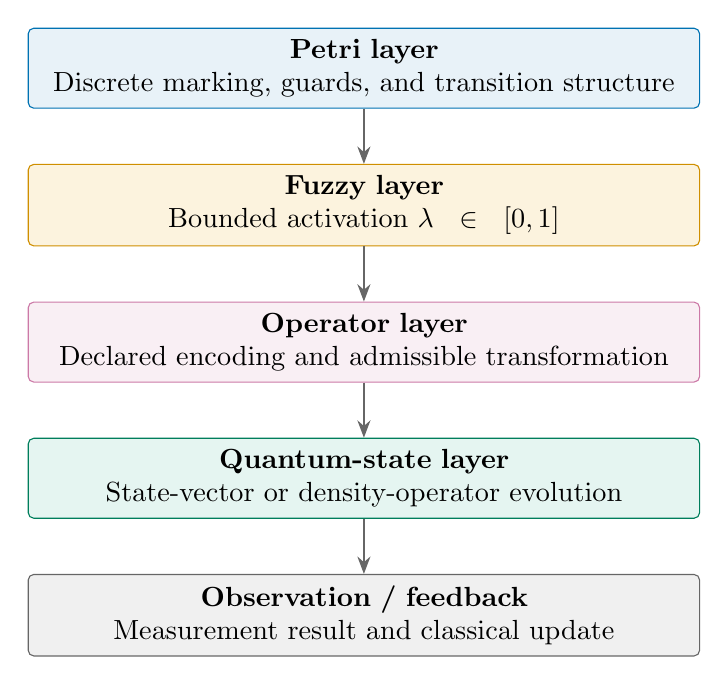
\begin{tikzpicture}[node distance=7mm, every node/.style={rounded corners=2pt, text width=0.68\linewidth, align=center, minimum height=8mm, inner sep=4pt}, link/.style={-{Stealth[length=2.2mm]}, thick, draw=QFLPNGrayCB}]
      \node[draw=QFLPNBlueCB, fill=QFLPNBlueCB!9] (petri) {\textbf{Petri layer}\\Discrete marking, guards, and transition structure};
      \node[draw=QFLPNOrangeCB!90!black, fill=QFLPNOrangeCB!13] [below=of petri] (fuzzy) {\textbf{Fuzzy layer}\\Bounded activation $\lambda\in[0,1]$};
      \node[draw=QFLPNPurpleCB, fill=QFLPNPurpleCB!12] [below=of fuzzy] (operator) {\textbf{Operator layer}\\Declared encoding and admissible transformation};
      \node[draw=QFLPNGreenCB!80!black, fill=QFLPNGreenCB!10] [below=of operator] (quantum) {\textbf{Quantum-state layer}\\State-vector or density-operator evolution};
      \node[draw=QFLPNGrayCB, fill=QFLPNGrayCB!10] [below=of quantum] (measure) {\textbf{Observation / feedback}\\Measurement result and classical update};
      \draw[link] (petri)--(fuzzy); \draw[link] (fuzzy)--(operator); \draw[link] (operator)--(quantum); \draw[link] (quantum)--(measure);
    \end{tikzpicture}
    \caption{Layered QFLPN semantic interface. Arrows denote declared mappings; they do not identify fuzzy activation, quantum amplitude, and measurement probability.}
    \label{fig:qflpn-architecture-overview}
\end{figure}
 This separation follows standard scientific manuscript practice in which methodology, obtained results, interpretation, and limitations are kept distinguishable \cite{ref6,ref7}.

\section{Research Context and Problem Definition}

\subsection{Discrete-event and quantum modelling context}

Quantum computation is commonly expressed through state vectors, density operators, unitary operators, and quantum channels, with experimental characterization of quantum dynamics requiring an explicit operator-level specification \cite{ref16}. Petri-net formalisms provide a complementary structural representation in which places and transitions express state storage and events. Previous QPN research has used this representation for quantum programs, quantum evolutionary systems, and quantum-centric dynamic applications \cite{ref3,ref5,ref4}. These developments motivate a framework in which a transition can carry both logical structure and a parameterized quantum transformation.

The QFLPN construction differs from a purely quantum Petri Net because the transition enabling mechanism contains an explicit fuzzy layer. Conversely, it differs from a fuzzy Petri Net because the state associated with a quantum-enabled place is not merely a scalar membership value. The formalism must therefore describe two coupled but non-identical state spaces: the discrete/fuzzy control space and the quantum state space.

\subsection{Semantic gap}

The central semantic gap can be stated precisely. Let $\mu\in[0,1]$ be a fuzzy membership value and let $|\psi\rangle\in\mathcal{H}$ be a quantum state. There is no mathematical identity
\begin{equation}
    \mu \equiv |\langle 1|\psi\rangle|^2
\end{equation}
without an explicitly defined encoding and state preparation. A QFLPN model must instead define a mapping
\begin{equation}
    \Gamma:[0,1]\rightarrow\mathcal{P},
\end{equation}
where $\mathcal{P}$ is a parameter space for admissible quantum operators. The particular choice of $\Gamma$ is part of the model specification.

This distinction prevents a common category error. Fuzzy activation expresses graded logical or inferential relevance; quantum amplitudes are complex coefficients of a state vector; probabilities are obtained from a state and a measurement prescription. The three quantities can be related, but they are not interchangeable by notation alone.

\subsection{Research question and scope}

The research question is: how can a formalism combine Petri-net structure, fuzzy activation, and quantum-state evolution while preserving the semantic distinction between these layers and providing directly testable mathematical invariants?

The scope of this article is the formal answer. The paper defines the model, transition semantics, operator interface, analytical properties, a reference four-qubit construction, and a reproducibility protocol. Large-scale sparse benchmarks, Taylor and Krylov comparisons, integral operators, degradation, decoherence, spectral convergence, tensor-network comparisons, and application-level validation are deliberately outside the evidentiary scope of this paper.

\section{Notation Summary}
Table~\ref{tab:p1-notation-summary} collects the principal symbols used throughout the formal development. Local symbols may acquire transition or subsystem indices when the relevant scope is clear from context.

\begin{longtable}{@{}p{0.24\linewidth}p{0.69\linewidth}@{}}
\caption{Principal notation used in this article.}\label{tab:p1-notation-summary}\\
\toprule
\textbf{Symbol} & \textbf{Meaning}\\
\midrule
\endfirsthead
\toprule
\textbf{Symbol} & \textbf{Meaning}\\
\midrule
\endhead
$\mathcal{N}_{\mathrm{QFLPN}}=(P,T,E,\mathcal{H},\mathcal{F})$ & QFLPN tuple: places, transitions, structural relation, Hilbert-space collection, and fuzzy mechanism.\\
$q$ & Number of qubits in the declared quantum register.\\
$d_p$ & Local Hilbert-space dimension associated with subsystem or place $p$.\\
$D$ & Dimension of the global Hilbert space; for $q$ qubits, $D=2^q$.\\
$M$ & Complete marking, including the relevant discrete/fuzzy information and quantum state.\\
$A_{\mathrm{str}}$ & Structural admissibility predicate for a transition and marking.\\
$A_{\mathrm{fz}}$ & Fuzzy activation value returned by the declared activation rule.\\
$A_{\tau}$ & Threshold-based activation or admissibility indicator, where that threshold rule is invoked.\\
$\lambda_t$ & Fuzzy activation associated with transition $t$, ordinarily in $[0,1]$.\\
$\tau$ & Declared fuzzy threshold used by a threshold-based rule.\\
$\vartheta_t$ & Operator parameter associated with transition $t$.\\
$\Gamma_t$ & Mapping from activation and declared parameters to the operator-parameter domain.\\
$K_{t,a}$ & Kraus operator indexed by $a$ for an open-system transition or quantum channel.\\
$\Pi_y$ & Measurement projector associated with outcome $y$.\\
$p_y$ & Probability of measurement outcome $y$ under the declared state and measurement.\\
$U_{\Sigma}$ & Global unitary operator formed from the declared local or transition operators, when the closed-system assumptions apply.\\
$\Phi_{\Sigma}$ & Global quantum evolution map; for open systems it may be a completely positive trace-preserving (CPTP) map.\\
$I(\rho)$ & A state invariant or diagnostic functional evaluated on density operator $\rho$; the specific invariant is stated at each use.\\
$\rho$ & Quantum density operator (state representation).\\
$\mathsf{M}$ & Declared measurement/observation convention, distinguished from the marking $M$ by font.\\
\bottomrule
\end{longtable}

\section{Formal QFLPN Architecture}

\subsection{QFLPN tuple}

Let the Quantum-Fuzzy Logical Petri Net be represented by
\begin{equation}
    \QFLPN=(P,T,E,\mathcal{H},\mathcal{F}),
\end{equation}
where $P$ is the set of places, $T$ is the set of transitions, $E$ is the structural relation connecting places and transitions, $\mathcal{H}$ is the collection of Hilbert spaces associated with quantum-enabled components, and $\mathcal{F}$ is the fuzzy activation mechanism.

For a concrete instance, the structural relation can be represented by directed arcs with application-specific weights or labels. The abstract tuple intentionally does not force one arc semantics, because the same operator interface can be implemented with ordinary, weighted, inhibitor, timed, or application-specific relations provided that transition admissibility is defined explicitly.

The complete marking is written as
\begin{equation}
    M=(M_C,M_F,M_Q),
\end{equation}
where $M_C$ contains discrete or classical place information, $M_F$ contains the fuzzy memberships relevant to enabled transitions, and $M_Q$ assigns a valid density operator to each quantum-enabled place. Thus the three state descriptions are typed objects rather than interchangeable scalar labels. A transition $t\in T$ is admissible only after its structural predicate and declared fuzzy activation have been evaluated; the quantum transformation is then selected through the operator map $\Gamma$.

\subsection{Semantic layers}

The architecture is separated into four operational layers. The structural layer contains the Petri-net topology and determines which places are connected to each transition. The fuzzy layer evaluates activation from the relevant memberships. The operator layer maps the activation and other parameters to an admissible quantum transformation. The state layer applies the transformation to the local or global quantum state.

\begin{figure}[tbp]
    \centering
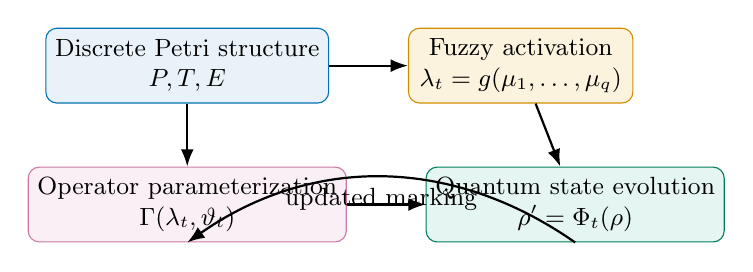
\begin{tikzpicture}[node distance=8mm and 10mm, every node/.style={font=\small}, block/.style={rounded corners, align=center, minimum width=2.85cm, minimum height=0.95cm}, arrow/.style={-{Latex[length=2.2mm]}, thick}]
        \node[block,draw=QFLPNBlueCB,fill=QFLPNBlueCB!9] (pn) {Discrete Petri structure\\$P,T,E$};
        \node[block,draw=QFLPNOrangeCB!90!black,fill=QFLPNOrangeCB!13, right=of pn] (fz) {Fuzzy activation\\$\lambda_t=g(\mu_1,\ldots,\mu_q)$};
        \node[block,draw=QFLPNPurpleCB,fill=QFLPNPurpleCB!12, below=of pn] (op) {Operator parameterization\\$\Gamma(\lambda_t,\vartheta_t)$};
        \node[block,draw=QFLPNGreenCB!80!black,fill=QFLPNGreenCB!10, right=of op] (qs) {Quantum state evolution\\$\rho' = \Phi_t(\rho)$};
        \draw[arrow] (pn) -- (fz);
        \draw[arrow] (fz) -- (qs);
        \draw[arrow] (op) -- (qs);
        \draw[arrow] (pn) -- (op);
        \draw[arrow,bend right=35] (qs.south) to node[below]{updated marking} (op.south);
\end{tikzpicture}
    \caption{Semantic architecture of the QFLPN model. The four layers are coupled through explicit interfaces rather than by identifying their state variables.}
    \label{fig:qflpn-architecture}
\end{figure}

The architecture is cyclic because the resulting quantum state may influence subsequent enabling or measurement conditions. The cycle does not imply that every implementation must measure the quantum state after every transition. It states only that the model admits feedback from state evolution to subsequent transition conditions when the application requires it.

\subsection{Local and global quantum markings}

For every quantum-enabled place $p\in P$, let $\mathcal{H}_p$ denote its local Hilbert space. The local quantum marking is represented by a density operator in
\begin{equation}
    \mathcal{M}_Q(p)\in\Dens(\mathcal{H}_p).
\end{equation}
For a composite system, the global Hilbert space is
\begin{equation}
    \Hglob=\bigotimes_{p\in P}\mathcal{H}_p.
\end{equation}

If the local dimensions are $d_p=\dim(\mathcal{H}_p)$, the global dimension is
\begin{equation}
    D=\prod_{p\in P}d_p.
\end{equation}
For $q$ qubits, $d_p=2$ for each qubit and therefore
\begin{equation}
    D=2^q.
\end{equation}
This distinction is retained throughout the paper: $q$ denotes the number of qubits, while $D$ denotes the dimension of the associated Hilbert space.

\subsection{Density-operator admissibility}

A density operator $\rho$ must satisfy
\begin{equation}
    \rho\succeq0,
    \qquad
    \rho=\rho^\dagger,
    \qquad
    \operatorname{Tr}(\rho)=1.
\end{equation}
The three constraints have different verification roles. Positive semidefiniteness guarantees non-negative probabilities for projective measurements. Hermiticity guarantees that expectation values of Hermitian observables are real. Unit trace normalizes the total probability.

These are formal admissibility conditions, not experimental observations. A numerical implementation can test their residuals, but a numerical test does not redefine the conditions themselves.

\section{Fuzzy Activation and Operator Encoding}

\subsection{Activation function}

For transition $t\in T$, let the relevant fuzzy memberships be $\mu_1(t),\ldots,\mu_q(t)$. The transition activation is
\begin{equation}
    \lambda_t=g\bigl(\mu_1(t),\ldots,\mu_q(t)\bigr),
\end{equation}
with the explicit requirement
\begin{equation}
    0\leq\lambda_t\leq1.
\end{equation}
The function $g$ belongs to the fuzzy layer. It may represent an application-specific aggregation rule, but its definition must be supplied for each concrete implementation.

The bound on $\lambda_t$ is important because the reference quantum encoding uses the square root of the activation. If a computational implementation produces a value outside the interval, the model must either reject the transition or explicitly define a normalization or saturation mechanism. Silent clipping would change the semantics and should not be introduced without being part of the model.

\subsection{Reference activation-to-rotation map}

For the reference QFLPN encoding, the activation is mapped to a rotation angle according to
\begin{equation}
    \theta_t=2\arcsin\sqrt{\lambda_t}.
\end{equation}
The corresponding single-qubit rotation is
\begin{equation}
    R_Y(\theta_t)=
    \begin{bmatrix}
        \cos(\theta_t/2) & -\sin(\theta_t/2) \\
        \sin(\theta_t/2) & \cos(\theta_t/2)
    \end{bmatrix}.
\end{equation}
For the initial state $|0\rangle$,
\begin{equation}
    R_Y(\theta_t)|0\rangle
    =
    \cos(\theta_t/2)|0\rangle
    +
    \sin(\theta_t/2)|1\rangle.
\end{equation}
Consequently, under this specific preparation and measurement convention,
\begin{equation}
    \Pr(1)=\sin^2(\theta_t/2)=\lambda_t.\label{eq:p1-reference}
\end{equation}
This equality is a property of the declared encoding and initial state; it is not a definition of fuzzy membership in general.

\subsection{Alternative encodings}

The formalism permits an alternative mapping
\begin{equation}
    \Gamma:[0,1]\times\Theta\rightarrow\mathcal{U},
\end{equation}
where $\Theta$ denotes additional classical parameters and $\mathcal{U}$ is the set of admissible unitary operators. An alternative encoding is acceptable only if its domain, range, state preparation, operator action, and verification conditions are declared. The existence of alternatives is useful for future comparative studies but does not weaken the status of the reference mapping used in this article.

\section{Transition Admissibility and Firing Semantics}

\subsection{Structural enabling}

A transition $t\in T$ is structurally admissible when the marking satisfies the input conditions associated with its incoming arcs. Denote the structural predicate by
\begin{equation}
    A_{\mathrm{str}}(t,M)=1.
\end{equation}
The exact predicate depends on the Petri-net interpretation of the arcs and tokens. The essential requirement is that the structural condition be evaluated before the quantum operator is applied.

\subsection{Fuzzy enabling}

The fuzzy condition is represented by
\begin{equation}
    A_{\mathrm{fz}}(t,M)=\lambda_t,
    \qquad
    \lambda_t\in[0,1].
\end{equation}
A thresholded implementation may introduce a declared parameter $\tau\in[0,1]$ and define an admissibility predicate
\begin{equation}
    A_{\tau}(t,M)=\mathbf{1}_{\{\lambda_t\geq\tau\}}.
\end{equation}
The threshold is optional. If it is not part of the application, the activation remains a graded parameter rather than a Boolean firing condition.

\subsection{Quantum transformation}

For a closed quantum subsystem, transition firing applies a unitary operator $U_t$:
\begin{equation}
    \rho' = U_t\rho U_t^\dagger,
    \qquad
    U_t^\dagger U_t=I.
\end{equation}
For an open subsystem, the more general representation is a completely positive trace-preserving map
\begin{equation}
    \rho'=\Phi_t(\rho).
\end{equation}
A Kraus representation can be written as
\begin{equation}
    \Phi_t(\rho)=\sum_a K_{t,a}\rho K_{t,a}^\dagger,
\end{equation}
with
\begin{equation}
    \sum_a K_{t,a}^\dagger K_{t,a}=I.
\end{equation}
This extension is essential when later studies include noise, decoherence, or degradation. This article defines the interface but does not claim measured decoherence performance.

\subsection{Partial observation and subsystem evolution}

When only a subsystem is observed, the reduced state is obtained by the partial trace. For a bipartite state $\rho_{AB}$,
\begin{equation}
    \rho_A=\operatorname{Tr}_B(\rho_{AB}).
\end{equation}
This operation permits a QFLPN model to maintain a global state while exposing only the information required by a classical controller or another transition. The distinction between the global state and a reduced state must remain explicit because entanglement can make a reduced state mixed even when the global state is pure.

\section{Operator Semantics and Analytical Properties}

\subsection{Unitary preservation of trace}

For $\rho'=U\rho U^\dagger$ and unitary $U$,
\begin{equation}
    \operatorname{Tr}(\rho')
    =\operatorname{Tr}(U\rho U^\dagger)
    =\operatorname{Tr}(U^\dagger U\rho)
    =\operatorname{Tr}(\rho)=1.
\end{equation}
Thus trace normalization is analytically preserved.

\subsection{Hermiticity preservation}

If $\rho=\rho^\dagger$, then
\begin{equation}
    (U\rho U^\dagger)^\dagger
    =U\rho^\dagger U^\dagger
    =U\rho U^\dagger.
\end{equation}
Hermiticity is therefore preserved exactly by unitary evolution.

\subsection{Positive semidefiniteness preservation}

For any vector $|v\rangle$, define $|w\rangle=U^\dagger|v\rangle$. Then
\begin{equation}
    \langle v|\rho'|v\rangle
    =\langle v|U\rho U^\dagger|v\rangle
    =\langle w|\rho|w\rangle
    \geq0,
\end{equation}
provided $\rho\succeq0$. Hence positive semidefiniteness is preserved.

\subsection{CPTP preservation}

For the open-system map $\Phi_t$, complete positivity and trace preservation imply that valid density operators are mapped to valid density operators. The trace-preserving property follows directly from the Kraus completeness relation:
\begin{equation}
    \operatorname{Tr}(\Phi_t(\rho))
    =\sum_a\operatorname{Tr}(K_{t,a}\rho K_{t,a}^\dagger)
    =\operatorname{Tr}\left(\rho\sum_aK_{t,a}^\dagger K_{t,a}\right)
    =\operatorname{Tr}(\rho).
\end{equation}
The complete-positivity requirement concerns positivity under extension with arbitrary ancillary systems and is the appropriate mathematical condition for a physical quantum channel.

\subsection{Observable probabilities}

For a projective measurement with projector $\Pi$, the probability is
\begin{equation}
    p(\Pi)=\operatorname{Tr}(\Pi\rho).
\end{equation}
The expression demonstrates why measurement probability belongs to the quantum layer. It depends on both the state and the measurement operator. A fuzzy membership value does not become a measurement probability unless the QFLPN instance explicitly constructs an encoding for which the equality holds.

\section{Transition Semantics and Formal Execution}\label{sec:step}

\noindent\textbf{Definition 1 (QFLPN step).} Let $\mathcal N=(P,T,E,\mathcal H,\mathcal F,\Gamma,\Phi,\mathcal M)$ be a QFLPN and let $M=(M_C,M_F,\rho)$ be a marking whose quantum component is a global density operator $\rho\in\mathcal D(\mathcal H_{\mathrm{glob}})$; the local markings are its marginals (Section~\ref{sec:consistency}). For a transition $t\in T$ the step $\mathrm{Step}_t$ is the partial map $M\mapsto(M',y)$ defined by the following stages, executed in this order. If a stage is undefined, $\mathrm{Step}_t$ is undefined at $M$: the transition does not fire, the marking, including the tokens of the input places, is left unchanged, and no rollback is needed.
\begin{enumerate}
\item[(S1)] \emph{Structural admissibility:} $A_{\mathrm{str}}(t,M_C)=1$. A failure is a structural failure.
\item[(S2)] \emph{Fuzzy aggregation:} $\lambda_t=g_t\big(\mu_1(t),\ldots,\mu_q(t)\big)\in[0,1]$, with $\mu_i(t)$ read from $M_F$; if a threshold $\tau$ is declared, additionally $\lambda_t\ge\tau$. A failure is a semantic failure.
\item[(S3)] \emph{Encoding:} $\vartheta_t=\Gamma_t(\lambda_t,\xi_t)\in\Theta_t$, the parameter domain of $\Phi_t$.
\item[(S4)] \emph{Quantum update:} $\rho'=\Phi_t(\rho;\vartheta_t)$, where $\Phi_t(\cdot\,;\vartheta)$ is a unitary conjugation or a CPTP map for every $\vartheta\in\Theta_t$. A failure is an operator failure.
\item[(S5)] \emph{Classical and fuzzy update:} $M_C'=F_t^{C}(M_C)$ and $M_F'=F_t^{F}(M_F)$, with declared rules (the identity when the memberships are supplied externally).
\item[(S6)] \emph{Optional observation:} an outcome $y$ of the observation map $\mathcal M_t$ on $\rho'$, obtained with probability $p_y=\mathrm{Tr}(\Pi_y\rho')$; if a feedback rule $G$ is declared, $M_C'\leftarrow G(M_C',y)$, otherwise $M_C'$ is unchanged.
\end{enumerate}
The result is $M'=(M_C',M_F',\rho')$.

\noindent\textbf{Proposition W (well-posedness of the step).} If $\rho\in\mathcal D(\mathcal H_{\mathrm{glob}})$ and stages (S1)--(S4) are defined, then $\rho'\in\mathcal D(\mathcal H_{\mathrm{glob}})$. If $\mathrm{Step}_{t_1},\ldots,\mathrm{Step}_{t_k}$ are defined in sequence, then $\rho_k=(\Phi_{t_k}\circ\cdots\circ\Phi_{t_1})(\rho_0)\in\mathcal D(\mathcal H_{\mathrm{glob}})$.

\noindent\textit{Proof.} By (S4) every $\Phi_t(\cdot\,;\vartheta)$ is CPTP, unitary conjugation being a special case, and a CPTP map sends density operators to density operators. A finite composition of CPTP maps is CPTP (Section~\ref{sec:cptp-closure}). $\square$

\noindent\textit{Reading guide.} The remaining results are statements about Definition~1. State validity and CPTP closure concern (S4); the reference encoding and its probability identity concern (S2)--(S3); ordering and concurrency concern the composition of steps; measurement and feedback concern (S6). The contract $C_t$ of Section~\ref{sec:contract} lists the components of the step.

\subsection{Composed transitions}

If a transition contains several local quantum operations acting on disjoint subsystems, the operator can be constructed as a tensor product,
\begin{equation}
    U_t=U_{t,1}\otimes U_{t,2}\otimes\cdots\otimes U_{t,r}.
\end{equation}
When the transition contains a controlled interaction, the operator is not factorized and must be specified directly or through a circuit decomposition. The formalism therefore accommodates both independent and coupled quantum actions without changing the Petri-net interface.

\subsection{Sequential composition}

For two admissible transitions $t_a$ and $t_b$, sequential execution is represented by
\begin{equation}
    \rho_2=\Phi_{t_b}\!\left(\Phi_{t_a}(\rho_0)\right).
\end{equation}
In the closed-system case this becomes
\begin{equation}
    \rho_2=U_{t_b}U_{t_a}\rho_0U_{t_a}^\dagger U_{t_b}^\dagger.
\end{equation}
The order is mathematically relevant whenever $U_{t_a}$ and $U_{t_b}$ do not commute. Specifically, in this operational semantics, $\rho_2=\Phi_{t_b}(\Phi_{t_a}(\rho_0))$ establishes that transition $t_a$ fires first and transition $t_b$ fires second. The reversed execution order evaluates to $\Phi_{t_a}(\Phi_{t_b}(\rho_0))$. The two sequential trajectories coincide if and only if $[U_{t_a},U_{t_b}]=0$ in the unitary regime, or when the corresponding superoperators commute in the open-system setting. This provides a precise link between Petri-net precedence and non-commutative quantum operator composition.

\subsection{Reachability representation}

Let $\mathcal{R}(M_0)$ denote the set of markings reachable from an initial marking $M_0$ through admissible transition sequences. A reachable execution path has the form
\begin{equation}
    M_0 \xrightarrow{t_1} M_1 \xrightarrow{t_2} M_2 \xrightarrow{t_3} \cdots \xrightarrow{t_k} M_k.
\end{equation}
Unlike a finite Boolean Petri-net state graph, the QFLPN reachability space may contain continuous quantum states and continuously varying fuzzy parameters. Therefore, a numerical implementation should distinguish logical reachability from sampled numerical trajectories. The former is a semantic property of the model; the latter is an experimental or computational observation.

\begin{figure}[tbp]
    \centering
    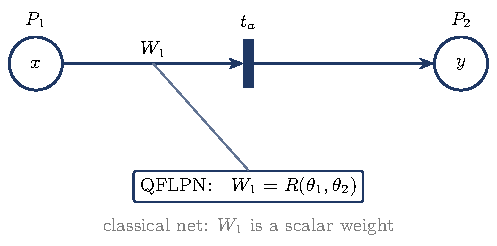
\includegraphics[width=0.78\linewidth]{figA_minimal_qflpn.pdf}
    \caption{Minimal QFLPN (model). Place $P_1$ holds $x$ and place $P_2$ holds $y$. The arc weight $W_1$ of a classical Petri net is a scalar; in a QFLPN it is the operator $R(\theta_1,\theta_2)$ whose parameters are produced by the encoding $\Gamma$ of the fuzzy activation of the transition $t_a$, so that the marking of $P_2$ results from the marking of $P_1$ through this operator.}
    \label{fig:qflpn-petri-motif}
\end{figure}

\section{Structural Properties and Propositions}

\subsection{Proposition on closed-system state validity}

\textbf{Proposition 1.} If $\rho$ is a valid density operator and $U$ is unitary, then $\rho'=U\rho U^\dagger$ is a valid density operator.

\textbf{Proof.} Hermiticity follows from
\begin{equation}
    (U\rho U^\dagger)^\dagger=U\rho U^\dagger.
\end{equation}
Trace preservation follows from cyclicity of the trace and $U^\dagger U=I$. Positive semidefiniteness follows because, for every vector $|v\rangle$, the quadratic form $\langle v|U\rho U^\dagger|v\rangle$ equals $\langle w|\rho|w\rangle$ for $|w\rangle=U^\dagger|v\rangle$. Therefore all three density-operator conditions are preserved. $\square$

\subsection{Proposition on sequential unitary composition}

\textbf{Proposition 2.} If $U_a$ and $U_b$ are unitary, then the sequential transition operator $U_bU_a$ is unitary.

\textbf{Proof.}
\begin{equation}
    (U_bU_a)^\dagger(U_bU_a)
    =U_a^\dagger U_b^\dagger U_bU_a
    =U_a^\dagger U_a
    =I.
\end{equation}
Thus the composition remains an admissible closed-system quantum transformation. $\square$

\subsection{Proposition on the reference encoding}

\textbf{Proposition 3.} For $\lambda\in[0,1]$, the reference parameter $\theta=2\arcsin\sqrt{\lambda}$ is real and satisfies $0\leq\theta\leq\pi$.

\textbf{Proof.} Since $0\leq\lambda\leq1$, one has $0\leq\sqrt{\lambda}\leq1$. Therefore $\arcsin\sqrt{\lambda}\in[0,\pi/2]$, giving $\theta\in[0,\pi]$. $\square$

\subsection{Proposition on fuzzy--quantum interface consistency}

\textbf{Proposition 4.} Under the declared reference encoding, if $\lambda\in[0,1]$, the operator $R_Y(2\arcsin\sqrt{\lambda})$ is unitary and, for the initial state $\lvert0\rangle$ followed by computational-basis measurement, the probability of outcome $1$ is exactly $\lambda$.

\textbf{Proof.} The matrix $R_Y(\theta)$ is real orthogonal and hence unitary for every real $\theta$. Proposition 3 guarantees that $\theta=2\arcsin\sqrt{\lambda}$ is real. Moreover,
\begin{equation}
    R_Y(\theta)\lvert0\rangle
    =\cos(\theta/2)\lvert0\rangle+\sin(\theta/2)\lvert1\rangle,
\end{equation}
so the outcome-$1$ probability is $\sin^2(\theta/2)=\lambda$. The equality follows from the declared encoding and does not identify fuzzy membership with a quantum amplitude.\ $\square$

These propositions establish formal properties that do not depend on a particular software implementation. They should be distinguished from numerical tests, which quantify floating-point residuals for a concrete implementation.

\section{QFLPN Structural Specification}

The formal definitions are summarized in Table~\ref{tab:qflpn-spec}. The purpose of this table is to make the model directly implementable: every object has a mathematical domain, a semantic role, and an evidence type. 

\begin{table}[tbp]
    \centering
    \caption{Formal specification of the principal QFLPN objects.}
    \label{tab:qflpn-spec}
\begin{tabular}{p{0.22\linewidth} p{0.28\linewidth} p{0.39\linewidth}}
        \toprule
        Object              & Mathematical form                                     & Semantic role                                                \\
        \midrule
        Net                 & $\mathcal{N}_{QFLPN}=(P,T,E,\mathcal{H},\mathcal{F})$ & Defines the complete model and its domains                   \\
        Structural relation & $E\subseteq(P\times T)\cup(T\times P)$                & Encodes precedence and connectivity                          \\
        Classical marking   & $M_C$                                                 & Stores discrete or classical state information               \\
        Fuzzy activation    & $\lambda_t=g(\mu_1,\ldots,\mu_q)$                     & Represents graded transition activation                      \\
        Local quantum state & $\rho_p\in\mathcal{D}(\mathcal{H}_p)$                 & Represents a quantum subsystem                               \\
        Global state        & $\rho\in\mathcal{D}(\mathcal{H}_{glob})$              & Represents the composite quantum system                      \\
        Operator map        & $\Gamma(\lambda_t,\xi_t)$                             & Converts declared classical parameters to quantum parameters \\
        Transition map      & $F_t$                                                 & Couples structural and quantum state updates                 \\
        Reachability        & $\mathcal{R}(M_0)$                                    & Describes markings accessible through admissible firings     \\
        \bottomrule
\end{tabular}\end{table}

\section{Reference Four-Qubit Instance}

\subsection{Dimension and basis convention}

The reference instance contains four qubits, hence
\begin{equation}
    q=4,
    \qquad
    D=2^4=16.
\end{equation}
The computational basis is ordered lexicographically from $|0000\rangle$ to $|1111\rangle$. The state representation therefore contains 16 complex amplitudes in the pure-state vector representation or a $16\times16$ density matrix in the mixed-state representation.

The basis convention is part of the reproducibility specification. A different tensor-product ordering may produce a different matrix layout even when the logical circuit is equivalent. The implementation must therefore document the qubit order before numerical outputs are interpreted.

\subsection{Activation-controlled rotations}

For each activation $\lambda_k$, the reference construction uses
\begin{equation}
    \theta_k=2\arcsin\sqrt{\lambda_k}
\end{equation}
and applies the corresponding $R_Y(\theta_k)$ operation to the declared qubit. The complete operator is constructed as a tensor product of local operators when the operations act independently, or as a controlled operator when the transition semantics require conditional coupling. Control-theoretic interpretations of such feedback interfaces can be related to classical stability and dissipativity frameworks \cite{ref17,ref18,ref19}.

\subsection{Controlled three-qubit condition}

For a three-control operation, define
\begin{equation}
    P_c=|111\rangle\langle111|.
\end{equation}
The controlled-X operator acting on the fourth qubit is
\begin{equation}
    C^3X=(I_8-P_c)\otimes I_2+P_c\otimes X.
\end{equation}
Here $P_c$ and $I_8$ act on the space of the three control qubits $q_1,q_2,q_3$, while $I_2$ and $X$ act on the fourth qubit $q_4$. Because $P_c$ and $I_8-P_c$ are orthogonal projectors that sum to $I_8$, the operator applies $X$ exactly on the $|111\rangle$ control subspace and the identity elsewhere.

\begin{figure}[tbp]
    \centering
\begin{tikzpicture}[x=1.05cm,y=0.85cm, every node/.style={font=\small}]
        \draw (0,3) -- (7,3);
        \draw (0,2) -- (7,2);
        \draw (0,1) -- (7,1);
        \draw (0,0) -- (7,0);
        \node[left] at (0,3) {$q_1$};
        \node[left] at (0,2) {$q_2$};
        \node[left] at (0,1) {$q_3$};
        \node[left] at (0,0) {$q_4$};
        \fill (3,3) circle (2.5pt);
        \fill (3,2) circle (2.5pt);
        \fill (3,1) circle (2.5pt);
        \draw (3,0) circle (6pt);
        \draw (2.94, -0.06) -- (3.06, 0.06);
        \draw (2.94, 0.06) -- (3.06, -0.06);
        \draw (3,1) -- (3,0);
        \draw (3,2) -- (3,0);
        \draw (3,3) -- (3,0);
        \node[above] at (3,3.15) {$|1\rangle$};
        \node[above] at (3,2.15) {$|1\rangle$};
        \node[above] at (3,1.15) {$|1\rangle$};
        \node[below] at (3,-0.25) {$X$};
        \node at (5.0,1.5) {$C^3X$};
\end{tikzpicture}
    \caption{Logical representation of the three-control operation used by the four-qubit reference construction.}
    \label{fig:c3x}
\end{figure}

\subsection{Reference state-space table}

\begin{table}[tbp]
    \centering
    \caption{Fixed conventions of the QFLPN four-qubit reference instance.}
    \label{tab:4q-conventions}
\begin{tabular}{p{0.36\linewidth} p{0.52\linewidth}}
        \toprule
        Property                & Reference convention                       \\
        \midrule
        Number of qubits        & $q=4$                                      \\
        Hilbert-space dimension & $D=16$                                     \\
        Basis                   & Computational basis, lexicographic order   \\
        State-vector precision  & Double precision                           \\
        Single-qubit encoding   & $\theta=2\arcsin\sqrt{\lambda}$            \\
        Reference rotation      & $R_Y(\theta)$                              \\
        Controlled operation    & $C^3X$                                     \\
        Control projector       & $P_c=|111\rangle\langle111|$               \\
        State representation    & Pure vector or density matrix, as declared \\
        Verification            & Trace, Hermiticity, positivity, dimension  \\
        \bottomrule
\end{tabular}
\end{table}

The table is not an experimental result. It is a fixed specification that allows two implementations to be compared under the same mathematical conventions.

\section{Scalability and Instance Hierarchy}

The four-qubit construction is a reference instance, not a scalability limit. The formalism is parameterized by the number of quantum subsystems and does not impose $q=4$. The value $q=4$ is selected because it is large enough to expose non-trivial controlled interaction while remaining small enough for exact, transparent verification of every matrix element. A scalable research program must distinguish this verification role from the computational regime used to study performance.

For an exact state-vector representation, the Hilbert-space dimension is
\begin{equation}
    D=2^q,
\end{equation}
and a dense complex-double state vector requires approximately $16\,2^q$ bytes, before auxiliary storage and implementation overhead are included. Consequently, the computational difficulty is governed exponentially by $q$ for generic exact state-vector simulation. For example, $q=20$ corresponds to $D=1,048,576$ amplitudes and approximately $16$ MiB for the state vector alone, whereas $q=30$ corresponds to approximately $16$ GiB and $q=40$ to approximately $16$ TiB. These figures are representation-level estimates, not measured QFLPN results.

\begin{table}[tbp]
    \centering
    \caption{Illustrative hierarchy of quantum-system sizes for exact state-vector representation.}
    \label{tab:scalability-hierarchy}
    \small
\begin{tabular}{>{\raggedright\arraybackslash}p{0.07\linewidth} >{\raggedright\arraybackslash}p{0.17\linewidth} >{\raggedright\arraybackslash}p{0.23\linewidth} >{\raggedright\arraybackslash}p{0.41\linewidth}}
        \toprule
        $q$ & $2^q$             & Approx. state-vector storage & Scientific role                           \\
        \midrule
        4   & 16                & 256 B                        & exact reference and semantic verification \\
        8   & 256               & 4 KiB                        & transition-composition tests              \\
        12  & 4096              & 64 KiB                       & controlled-interaction tests              \\
        16  & 65536             & 1 MiB                        & small numerical benchmark                 \\
        20  & 1,048,576         & 16 MiB                       & moderate exact benchmark                  \\
        30  & 1,073,741,824     & 16 GiB                       & large exact state-vector regime           \\
        40  & 1,099,511,627,776 & 16 TiB                       & memory-dominated regime                   \\
        \bottomrule
\end{tabular}
\end{table}

The hierarchy also clarifies why a statement such as ``10,000 qubits'' cannot be treated as a generic continuation of the four-qubit experiment. For a fully generic dense state-vector model, $q=10{,}000$ would require $2^{10{,}000}$ amplitudes and is therefore not an exact classical state-vector target. Large qubit counts become meaningful only after the representation and the structure being exploited are specified. Tensor-network methods, sparse representations, stabilizer methods, symmetry reductions, or other compressed descriptions can access substantially larger structured systems, but their achievable size depends on entanglement, topology, circuit depth, observable, approximation tolerance, and contraction strategy. Recent benchmarking literature explicitly shows that simulator choice and circuit structure can change feasibility by more than an order of magnitude, while tensor-network approaches have their own representation-dependent limits.\cite{ref1,ref2}

This distinction is essential for future investigations. Quantum-system size $q$, Petri-net size $(|P|,|T|)$, sparse matrix dimension $N$, and number of experimental repetitions are different quantities and must never be reported as interchangeable ``system size''. The reference instance in this article remains four-qubit. Future studies may use larger quantum instances when the selected representation and available evidence support them. A larger instance is scientifically valuable only when it tests a new hypothesis rather than merely increasing a numerical parameter.

\section{Worked Examples}\label{sec:examples}
\subsection{An open-system step: amplitude damping}
Take $\lambda=0.7$. The reference encoding gives $|\psi\rangle=\sqrt{0.3}\,|0\rangle+\sqrt{0.7}\,|1\rangle$ and $\Pr(1)=\lambda$. The amplitude-damping channel with parameter $\gamma\in[0,1]$ has the Kraus operators
\begin{equation}
 K_0=\begin{pmatrix}1&0\\0&\sqrt{1-\gamma}\end{pmatrix},\qquad
 K_1=\begin{pmatrix}0&\sqrt{\gamma}\\0&0\end{pmatrix},
\end{equation}
and $K_0^\dagger K_0+K_1^\dagger K_1=\mathrm{diag}(1,\,1-\gamma+\gamma)=I$, so the completeness relation holds. For $\rho=|\psi\rangle\langle\psi|$ the output is
\begin{equation}
 \rho'=\begin{pmatrix}1-(1-\gamma)\lambda & \sqrt{(1-\gamma)\lambda(1-\lambda)}\\ \sqrt{(1-\gamma)\lambda(1-\lambda)} & (1-\gamma)\lambda\end{pmatrix}.
\end{equation}
Its trace is $1$ and its determinant is $\gamma(1-\gamma)\lambda^2\ge0$, so $\rho'\succeq0$. Its purity is $\mathrm{Tr}\,\rho'^2=1-2\gamma(1-\gamma)\lambda^2$; for $\gamma=0.2$ this is $0.8432$, whereas unitary evolution keeps the purity equal to $1$.

The semantic consequence is that the identity $\Pr(1)=\lambda$ of the reference encoding is a property of the closed step. After the open step the readout is $\Pr(1)=(1-\gamma)\lambda=0.56$ for $\gamma=0.2$, which differs from the fuzzy activation by the factor $1-\gamma$. This is not a defect of the encoding but what the separation of the fuzzy and the quantum layers predicts. Phase damping, with Kraus operators $\sqrt{1-p}\,I$ and $\sqrt{p}\,Z$, behaves differently: the populations and hence $\Pr(1)=\lambda$ are unchanged, while the coherence is multiplied by $1-2p$, that is $\rho'=\begin{pmatrix}1-\lambda&(1-2p)\sqrt{\lambda(1-\lambda)}\\(1-2p)\sqrt{\lambda(1-\lambda)}&\lambda\end{pmatrix}$ (the other common Kraus form, $\mathrm{diag}(1,\sqrt{1-p'})$ and $\mathrm{diag}(0,\sqrt{p'})$, describes the same channel for $p'=4p(1-p)$ with $0\le p\le\tfrac12$); for $p=0.2$ it falls from $0.458$ to $0.275$ and the purity to $0.7312$.

The closed forms agree with the numerical channel to $9.2\times10^{-16}$ over $2000$ random pairs $(\lambda,\gamma)$. In $20000$ random draws of both channels the Choi matrix is positive semidefinite and the output is a density operator in every case (violations: $0$). An independent implementation with the \texttt{Kraus} and \texttt{DensityMatrix} classes of Qiskit confirms that both channels are CPTP and reproduces the outputs exactly.

\subsection{Concurrency versus commutativity}
Let $t_a$ apply $R_Y(\theta_a)$ to qubit $q_1$ with $\lambda_a=0.7$, and let $t_b$ be either $R_Y(\theta_b)$ on $q_2$ with $\lambda_b=0.4$ (disjoint quantum supports) or a controlled-NOT with control $q_1$ and target $q_2$ (overlapping supports). The initial state is $|00\rangle$ and the order dependence is measured by the trace-norm distance
\begin{equation}
 \Delta_\rho=\big\|U_bU_a\rho U_a^\dagger U_b^\dagger-U_aU_b\rho U_b^\dagger U_a^\dagger\big\|_1 .
\end{equation}
For disjoint supports $[U_a,U_b]=0$ and $\Delta_\rho=0$. For overlapping supports $\|[U_a,U_b]\|_F=2.366$ and $\Delta_\rho=1.908$. Analytically, firing $t_a$ first gives $\sqrt{1-\lambda_a}\,|00\rangle+\sqrt{\lambda_a}\,|11\rangle$, an entangled state, whereas firing $t_b$ first gives $\big(\sqrt{1-\lambda_a}\,|0\rangle+\sqrt{\lambda_a}\,|1\rangle\big)|0\rangle$; the squared fidelity is $(1-\lambda_a)^2=0.09$ and $\Delta_\rho=2\sqrt{1-F}=1.908$, as computed. The two transitions can be structurally concurrent in the Petri layer, with disjoint classical input places, and still produce firing-order-dependent states because they share the quantum subsystem $q_1$. Commutation follows from disjoint quantum support, not from Petri-net concurrency. The Qiskit computation agrees with the numerical one to within $6\times10^{-17}$.

\noindent\textbf{Proposition O (order dependence and the commutator).} For unitaries $U_a,U_b$ and a pure state $|\psi\rangle$,
\begin{equation}
 \Delta_\rho=2\sqrt{1-\big|\langle\psi|U_a^\dagger U_b^\dagger U_aU_b|\psi\rangle\big|^2}\;\le\;2\,\big\|[U_a,U_b]\big\|_{\mathrm{op}} .
\end{equation}
Hence $\Delta_\rho=0$ if and only if $|\psi\rangle$ is an eigenvector of the group commutator $U_a^\dagger U_b^\dagger U_aU_b$, and $\Delta_\rho=0$ for every state if and only if $U_aU_b=e^{i\varphi}U_bU_a$ for some phase $\varphi$.

\noindent\textit{Proof.} Let $|u\rangle=U_bU_a|\psi\rangle$ and $|v\rangle=U_aU_b|\psi\rangle$. For unit vectors, $\||u\rangle\langle u|-|v\rangle\langle v|\|_1=2\sqrt{1-|\langle u|v\rangle|^2}$, and $\langle u|v\rangle=\langle\psi|U_a^\dagger U_b^\dagger U_aU_b|\psi\rangle$, which gives the equality. With $c=|\langle u|v\rangle|$ one has $1-c^2\le2(1-c)\le\|u-v\|^2$, so $\Delta_\rho\le2\|u-v\|=2\|(U_bU_a-U_aU_b)|\psi\rangle\|\le2\|[U_a,U_b]\|_{\mathrm{op}}$. The group commutator $K$ is unitary, so $|\langle\psi|K|\psi\rangle|=1$ exactly when $K|\psi\rangle=e^{i\varphi}|\psi\rangle$; this holds for all $|\psi\rangle$ exactly when $K=e^{i\varphi}I$, that is, $U_aU_b=e^{i\varphi}U_bU_a$. $\square$

For the overlapping example above $\Delta_\rho=1.908$ and $\|[U_a,U_b]\|_{\mathrm{op}}=1.673$, so the bound $3.347$ holds without being tight. For $10000$ random pairs of $4\times4$ unitaries and random states the identity held to $4.4e-15$ and the bound was never violated. The proposition ties the order dependence of two firings to a norm of their commutator, which the structure of the net alone cannot supply.

\noindent\textbf{Corollary A (composition of amplitude-damping steps).} For the amplitude-damping channels of the previous subsection, $\mathcal A_{\gamma_2}\circ\mathcal A_{\gamma_1}=\mathcal A_{\gamma}$ with $\gamma=1-(1-\gamma_1)(1-\gamma_2)$. Consequently $k$ successive open steps with parameter $\gamma$ give $\Pr(1)=(1-\gamma)^k\lambda$.

\noindent\textit{Proof.} The products of the Kraus operators are $\mathrm{diag}\big(1,\sqrt{(1-\gamma_1)(1-\gamma_2)}\big)$, $\sqrt{\gamma_2(1-\gamma_1)}\,|0\rangle\langle1|$, $\sqrt{\gamma_1}\,|0\rangle\langle1|$ and $0$. The two jump operators are proportional to $|0\rangle\langle1|$ and merge into a single one with weight $\gamma_2(1-\gamma_1)+\gamma_1=1-(1-\gamma_1)(1-\gamma_2)$, which is the Kraus form of $\mathcal A_\gamma$. The population of $|1\rangle$ is multiplied by $1-\gamma_i$ at each step. $\square$

\noindent\textbf{Corollary B (composition of phase-damping steps).} For the phase-damping channel $\Phi_p(\rho)=(1-p)\rho+pZ\rho Z$ with $p\in[0,1]$, the composition satisfies $\Phi_{p_2}\circ\Phi_{p_1}=\Phi_p$ with $p=p_1+p_2-2p_1p_2\in[0,1]$. Consequently $k$ successive phase-damping steps maintain populations $\Pr(1)=\lambda$ invariant while attenuating off-diagonal coherence by $(1-2p)^k$.

\noindent\textit{Proof.} Expanding $\Phi_{p_2}(\Phi_{p_1}(\rho)) = (1-p_2)[(1-p_1)\rho+p_1Z\rho Z] + p_2 Z[(1-p_1)\rho+p_1Z\rho Z]Z$. Using $Z^2=I$, the coefficient of $\rho$ is $(1-p_2)(1-p_1)+p_2p_1 = 1-(p_1+p_2-2p_1p_2)$, while the coefficient of $Z\rho Z$ is $(1-p_2)p_1+p_2(1-p_1) = p_1+p_2-2p_1p_2$, which matches $\Phi_p$ with $p=p_1+p_2-2p_1p_2$. $\square$

\noindent\textbf{Proposition (Holevo capacity bound for the amplitude-damping step).} Let $\mathcal A_\gamma$ be the amplitude-damping channel with damping parameter $\gamma\in[0,1]$. For the equiprobable binary ensemble $\{1/2, |0\rangle\langle0|;\, 1/2, |1\rangle\langle1|\}$, the Holevo information is
\begin{equation}
    \chi(\gamma) = h\Big(\frac{1-\gamma}{2}\Big) - \frac{1}{2}h(1-\gamma),
\end{equation}
where $h(x)=-x\log_2 x - (1-x)\log_2(1-x)$ is the binary entropy function. The bound satisfies $\chi(0)=1$~bit (noiseless identity) and $\chi(1)=0$ (complete decoherence to ground state $|0\rangle$).

A numerical check of the composition law over $5000$ random pairs agrees with the Choi matrices to $8.4e-15$.

\subsection{Consistency of local and global states}\label{sec:consistency}
\noindent\textbf{Definition 2 (consistent quantum marking).} The quantum component of a marking is a global state $\rho\in\mathcal D(\mathcal H_{\mathrm{glob}})$; the local marking of a set $S$ of quantum places is $M_Q(S)=\mathrm{Tr}_{P\setminus S}\,\rho$. A family of local states given independently is admissible only if it consists of marginals of one global state.

\noindent\textbf{Proposition L (locality of marginals).} If a transition acts through a channel $\Phi$ on the subsystem $S$ only, that is, the global update is $\Phi\otimes\mathrm{id}$, then the marginal on the complement of $S$ is unchanged.

\noindent\textit{Proof.} For every operator $X$ on the complement, $\mathrm{Tr}\big[(I\otimes X)(\Phi\otimes\mathrm{id})(\rho)\big]=\mathrm{Tr}\big[(\Phi^\dagger(I)\otimes X)\rho\big]=\mathrm{Tr}[(I\otimes X)\rho]$, because trace preservation means $\Phi^\dagger(I)=I$. $\square$

\noindent\textbf{Proposition M (entangled marginals cannot be assigned independently).} If the marginal $\rho_{AB}$ of a state $\rho_{ABC}$ is pure, then $\rho_{ABC}=\rho_{AB}\otimes\rho_C$. Consequently no global state has two overlapping marginals $\rho_{AB}$ and $\rho_{BC}$ that are both pure and entangled.

\noindent\textit{Proof.} Write $\rho_{ABC}=\sum_kp_k|\chi_k\rangle\langle\chi_k|$. The marginals $\mathrm{Tr}_C|\chi_k\rangle\langle\chi_k|$ are positive and sum, with weights, to the rank-one operator $|\varphi\rangle\langle\varphi|=\rho_{AB}$, so each is proportional to it. A pure state on $AB\otimes C$ whose $AB$ marginal has rank one is a product $|\varphi\rangle\otimes|c_k\rangle$. Hence $\rho_{ABC}=|\varphi\rangle\langle\varphi|\otimes\rho_C$ and $\rho_{BC}=\rho_B\otimes\rho_C$ is a product state. $\square$

Definition~2 therefore excludes incompatible local assignments by construction. As a numerical illustration, for a Bell pair the marginal of $B$ is maximally mixed (purity $0.5$), and applying $1000$ random amplitude-damping or phase-damping channels to $A$ left it unchanged at double precision, as Proposition~L requires.

\subsection{An illustrative run of a small net}\label{sec:run}
The following design is illustrative and is not derived from an application. The net is $p_1\rightarrow t_1\rightarrow p_2\rightarrow t_2\rightarrow p_3$ with one classical token and two qubits, $a$ attached to $p_2$ and $b$ attached to $p_3$, both initially in $|0\rangle$. Transition $t_1$ aggregates two sources with memberships $(0.8,0.6)$ and weights $(0.5,0.5)$ into $\lambda_1=0.70$, encodes $\theta_1=1.9823$ and applies $R_Y(\theta_1)$ to $a$. Transition $t_2$ aggregates memberships $(0.9,0.5)$ with weights $(0.6,0.4)$ into $\lambda_2=0.74$, encodes $\theta_2=2.0715$ and applies a controlled $R_Y(\theta_2)$ to $b$ with control $a$. The run was computed in PennyLane and in numpy, which agree exactly at double precision. Table~\ref{tab:p1-run} and Fig.~\ref{fig:p1-run} give the marking and the quantum state after each firing.
\begin{table}[tbp]
\centering\small
\caption{Marking and quantum state in the illustrative run.}
\label{tab:p1-run}
\begin{tabular}{lcccc}
\toprule
Stage & Token in & $\Pr(a=1)$ & $\Pr(b=1)$ & Purity of $\rho_a$ \\
\midrule
Initial marking & $p_1$ & 0.000 & 0.000 & 1.000 \\
After $t_1$ & $p_2$ & 0.700 & 0.000 & 1.000 \\
After $t_2$ & $p_3$ & 0.700 & 0.518 & 0.689 \\
\bottomrule
\end{tabular}
\end{table}
\begin{figure}[tbp]
\centering
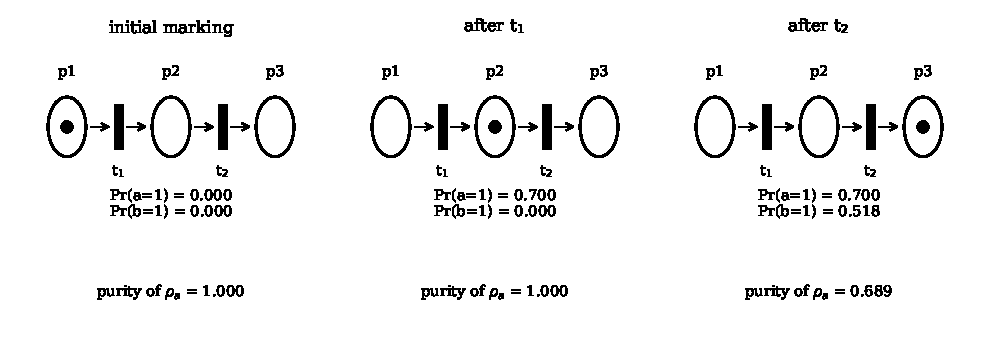
\includegraphics[width=0.98\linewidth]{fig_p1_net_example.pdf}
\caption{Illustrative run of a small QFLPN: classical marking (token), measurement probabilities of the two qubits, and purity of the reduced state of qubit $a$ after each firing.}
\label{fig:p1-run}
\end{figure}
The firing of $t_2$ leaves $\Pr(a=1)$ unchanged, because a controlled operation is diagonal in the computational basis of its control; it creates $\Pr(b=1)=\lambda_1\lambda_2=0.518$ and entangles the two qubits, as the purity $0.689$ of $\rho_a$ (von Neumann entropy $0.707$ bits) shows. The Petri-net order also matters: if $t_2$ fired before $t_1$ it would act on a control in $|0\rangle$ and change nothing, and the trace-norm distance between the two final states is $1.508$. The example makes the six stages of Definition~1 concrete: the token moves by (S1) and (S5), $\lambda_t$ is computed by (S2), $\theta_t$ by (S3), and the state changes by (S4).

\section{Formal Completeness and Execution Contract}\label{sec:contract}

The formal definitions above can be assembled into an execution contract that determines what must be specified before a QFLPN transition is considered mathematically well-defined. This contract is useful because the same Petri topology can otherwise admit different fuzzy aggregation rules, operator parameterizations, basis orderings, and measurement conventions. The model is therefore treated as a typed composition rather than as an informal correspondence between diagram elements.

For a transition $t$, define the semantic contract
\begin{equation}
    \mathfrak{C}_t=
    (A_{\mathrm{str}},g,\Gamma,\Phi,\mathsf{M}),
\end{equation}
where $A_{\mathrm{str}}$ is the structural admissibility predicate, $g$ is the fuzzy aggregation rule, $\Gamma$ is the activation-to-operator parameter map, $\Phi$ is the quantum transformation, and $\mathsf{M}$ is the declared measurement or observation convention. A transition specification is complete only when the domains and codomains of these components are fixed.

For the closed-system reference case, the contract can be expressed as
\begin{equation}
    M \xrightarrow{A_{\mathrm{str}}}
    \lambda_t
    \xrightarrow{\Gamma}
    \vartheta_t
    \xrightarrow{U_t(\vartheta_t)}
    \rho'
    \xrightarrow{\mathsf{M}}
    y,
\end{equation}
where $y$ denotes an optional classical observation. Each arrow has a distinct mathematical type. In particular, $\lambda_t$ is a scalar activation, $\vartheta_t$ is an operator parameter, $U_t$ is an operator, and $y$ is an observation produced only after a measurement or declared readout operation.

The contract also fixes the direction of dependence. The fuzzy value may parameterize a quantum operator, but the quantum state is not altered merely by computing $\lambda_t$. Conversely, a quantum measurement may influence a subsequent classical marking only when the model explicitly includes a feedback rule. This distinction prevents an implicit information transfer between semantic layers.

\subsection{Well-posed transition conditions}

A transition is well-posed when the following conditions hold simultaneously: the structural predicate is defined on the current marking; the fuzzy aggregation produces a value in $[0,1]$; the parameter map produces an element of its declared parameter space; and the quantum transformation maps admissible states to admissible states. For the unitary reference case this gives
\begin{equation}
    A_{\mathrm{str}}(t,M_C)=1,
    \qquad
    0\leq\lambda_t\leq1,
    \qquad
    U_t^\dagger U_t=I.
\end{equation}

These conditions separate three different failure modes. A structural failure means that the transition is not enabled. A semantic failure means that the fuzzy or parameterization layer produced an invalid value. An operator failure means that the declared transformation does not satisfy the admissibility conditions required by the selected quantum semantics. Treating these cases separately makes implementation diagnostics scientifically interpretable.

For the reference encoding $\theta_t=2\arcsin\sqrt{\lambda_t}$, the activation constraint alone guarantees
\begin{equation}
    0\leq\theta_t\leq\pi.
\end{equation}
The angle is therefore real and lies in the principal interval used by the stated single-qubit rotation convention. This is an analytical consequence of the encoding and does not require a numerical experiment.

\subsection{Invariants under repeated firing}

If a sequence of closed-system transitions is represented by unitary operators $U_1,\ldots,U_k$, the resulting state is
\begin{equation}
    \rho_k=U_k\cdots U_2U_1\rho_0U_1^\dagger U_2^\dagger\cdots U_k^\dagger.
\end{equation}
Because the product $U_k\cdots U_1$ is unitary, density-operator validity is preserved for the entire sequence. Thus trace normalization, Hermiticity, and positive semidefiniteness are invariants of repeated closed-system firing.

This invariant statement is stronger than checking one transition in isolation. It establishes that the local correctness condition composes over an arbitrary finite sequence, provided every transition in that sequence satisfies the declared unitary contract. For open-system transitions, the analogous statement follows from closure of CPTP maps under composition.

\subsection{Ordering, concurrency, and non-commutativity}

Petri-net concurrency does not automatically imply quantum-operator commutativity. Consider two transitions $t_a$ and $t_b$ with operators $U_a$ and $U_b$. If
\begin{equation}
    [U_a,U_b]=U_aU_b-U_bU_a=0,
\end{equation}
then the corresponding closed-system state transformations are order-independent at the operator level. If instead
\begin{equation}
    [U_a,U_b]\neq0,
\end{equation}
the execution order is semantically relevant and the two transition sequences generally produce different states.

For operations acting on disjoint tensor factors, commutativity follows from the tensor-product structure. If $U_a$ acts only on subsystem $A$ and $U_b$ only on subsystem $B$, then
\begin{equation}
    (U_a\otimes I_B)(I_A\otimes U_b)
    =
    (I_A\otimes U_b)(U_a\otimes I_B).
\end{equation}
This provides a precise mathematical criterion for identifying a class of QFLPN transitions that can be treated as independent concurrent actions. Controlled interactions, shared subsystems, and overlapping supports require the commutator or an equivalent operator relation to be evaluated explicitly.

\begin{figure}[tbp]
    \centering
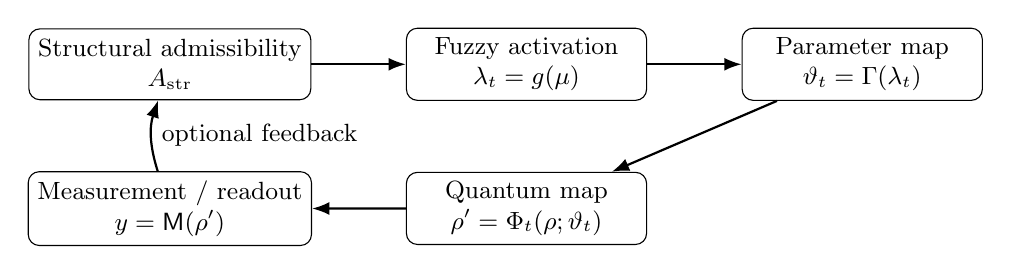
\begin{tikzpicture}[node distance=9mm and 12mm, every node/.style={font=\small}, block/.style={draw, rounded corners, align=center, minimum width=3.05cm, minimum height=0.9cm}, arrow/.style={-{Latex[length=2.2mm]}, thick}]
        \node[block] (s) {Structural admissibility\\$A_{\mathrm{str}}$};
        \node[block,right=of s] (f) {Fuzzy activation\\$\lambda_t=g(\mu)$};
        \node[block,right=of f] (g) {Parameter map\\$\vartheta_t=\Gamma(\lambda_t)$};
        \node[block,below=of f] (u) {Quantum map\\$\rho'=\Phi_t(\rho;\vartheta_t)$};
        \node[block,below=of s] (m) {Measurement / readout\\$y=\mathsf{M}(\rho')$};
        \draw[arrow] (s) -- (f);
        \draw[arrow] (f) -- (g);
        \draw[arrow] (g) -- (u);
        \draw[arrow] (u) -- (m);
        \draw[arrow,bend left=18] (m) to node[right]{optional feedback} (s);
\end{tikzpicture}
    \caption{Execution contract for a QFLPN transition. Feedback from a measurement to structural enabling is optional and must be explicitly defined by the model.}
    \label{fig:qflpn-execution-contract}
\end{figure}

\begin{figure}[tbp]
\centering
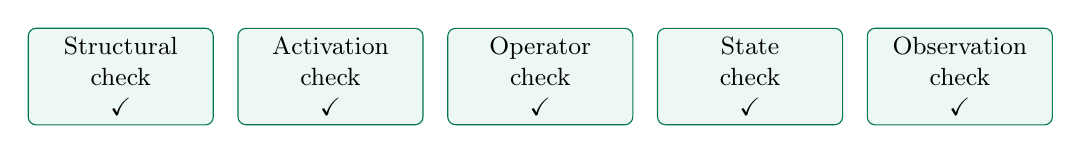
\begin{tikzpicture}[font=\small, node distance=3mm,
  check/.style={draw=QFLPNGreenCB!75!black,fill=QFLPNGreenCB!7,rounded corners=1mm,minimum width=2.35cm,minimum height=10mm,align=center},
  tick/.style={font=\large\bfseries\color{QFLPNGreenCB!80!black}}]
\node[check] (a) {Structural\\check\\{$\checkmark$}};
\node[check,right=of a] (b) {Activation\\check\\{$\checkmark$}};
\node[check,right=of b] (c) {Operator\\check\\{$\checkmark$}};
\node[check,right=of c] (d) {State\\check\\{$\checkmark$}};
\node[check,right=of d] (e) {Observation\\check\\{$\checkmark$}};
\end{tikzpicture}
\caption{Execution-contract checklist. Check marks denote verification obligations specified by the framework, not a claim that every possible implementation has been empirically tested.}
\label{fig:p1-execution-checklist}
\end{figure}


\subsection{Measurement and classical feedback}

Let $\\{\Pi_y\\}$ be a projective measurement satisfying
\begin{equation}
    \Pi_y=\Pi_y^\dagger,
    \qquad
    \Pi_y\Pi_z=0\quad(y\neq z),
    \qquad
    \sum_y\Pi_y=I.
\end{equation}
The probability of outcome $y$ is
\begin{equation}
    p_y=\operatorname{Tr}(\Pi_y\rho).
\end{equation}
If the QFLPN model uses this outcome to update a classical marking, a feedback function must be supplied explicitly, for example
\begin{equation}
    M_C'=G(M_C,y).
\end{equation}
The measurement therefore creates a well-defined interface from the quantum layer back to the discrete layer. Without a declared $G$, no classical state update should be inferred from the measurement merely because the measurement has been computed.

The same principle applies to partial observations. If $\rho_A=\operatorname{Tr}_B(\rho_{AB})$, then any controller using $\rho_A$ must specify which functional of $\rho_A$ is used for the next decision. This explicit controller interface is consistent with the broader control-theoretic separation between the plant state, measured information, and the feedback law \cite{ref17,ref18,ref19,ref20}. This keeps the information flow auditable and prevents a reduced-state calculation from being mistaken for a full-state observation.

\subsection{Formal verification obligations}

The mathematical model yields a compact set of verification obligations that can be tested independently of performance experiments. The structural obligation checks the declared input and output relation of each transition. The fuzzy obligation checks the domain and range of the activation function. The operator obligation checks unitarity for closed transitions or the CPTP conditions for open transitions. The state obligation checks density-operator admissibility after each firing. The interface obligation checks that basis ordering, subsystem support, and measurement conventions are identical between the mathematical specification and the implementation.

These obligations define what can be established analytically before any large-scale numerical benchmark is attempted. They also explain why a small deterministic instance is scientifically useful: it can validate the complete semantic chain without conflating correctness with computational performance.

\section{Computational Representation and Complexity}

\subsection{Dense representation}

For a $D$-dimensional pure state, a state vector requires $D$ complex amplitudes. A dense density matrix requires $D^2$ complex entries. For the four-qubit reference, $D=16$, so the dense state-vector representation contains 16 amplitudes and the density-matrix representation contains 256 complex entries. These quantities are exact consequences of the representation dimension.

\subsection{Sparse representation}

When the operator or state exhibits exploitable sparsity, a sparse representation can reduce storage and arithmetic cost. For a matrix in compressed sparse row representation, the cost of one sparse matrix-vector multiplication is proportional to the number of stored nonzero elements, conventionally denoted by $\mathrm{NNZ}$, together with lower-order indexing operations. This observation motivates separate computational studies of sparse storage and evolution.

\subsection{Complexity boundary}

The QFLPN tuple does not imply one universal computational complexity. Complexity depends on the state representation, operator structure, sparsity, algorithm, precision, hardware, and stopping criteria. A formal statement such as
\begin{equation}
    \text{QFLPN is scalable}
\end{equation}
would therefore be scientifically incomplete without specifying the computational regime and measured evidence. This article instead establishes the representation-level quantities from which such analyses can later be derived.

\section{Verification Framework}

\subsection{Analytical verification}

Analytical verification establishes properties that follow from the definitions. Examples include the preservation of trace, Hermiticity and positive semidefiniteness under unitary evolution, and trace preservation under a CPTP map. These results are independent of a particular programming language or processor.

\subsection{Numerical verification}

Numerical verification evaluates a concrete implementation. The following residuals are directly relevant:
\begin{equation}
    \varepsilon_{\mathrm{tr}}=|\operatorname{Tr}(\rho)-1|,
\end{equation}
\begin{equation}
    \varepsilon_{\mathrm{H}}=\|\rho-\rho^\dagger\|,
\end{equation}
and a positive-semidefiniteness diagnostic based on the minimum eigenvalue,
\begin{equation}
    \varepsilon_{\mathrm{PSD}}=\max\{0,-\lambda_{\min}(\rho)\}.
\end{equation}
The matrix norm used for $\varepsilon_{\mathrm{H}}$ and the numerical tolerance must be declared by the implementation. A result is reproducible only when these conventions are fixed.

\subsection{Independent implementation check}

A stronger verification protocol uses two independent implementations with the same input parameters and basis ordering. Agreement of the final state or declared observables within a pre-specified tolerance provides evidence of implementation consistency. It does not prove physical correctness in an experimental processor, but it substantially reduces the risk of a hidden implementation-specific error.

\begin{table}[tbp]
    \centering
    \caption{Verification layers for the formal QFLPN framework.}
    \label{tab:verification}
\begin{tabular}{p{0.24\linewidth} p{0.31\linewidth} p{0.33\linewidth}}
        \toprule
        Layer              & Object tested                  & Evidence type                      \\
        \midrule
        Formal             & Tuple, domains, codomains      & Definition and derivation          \\
        Operator           & Unitarity or CPTP conditions   & Algebraic verification             \\
        State              & Trace, Hermiticity, positivity & Analytical and numerical residuals \\
        Reference instance & Dimension and basis ordering   & Deterministic specification        \\
        Implementation     & Independent output agreement   & Reproducible numerical test        \\
        Physical system    & Hardware execution and noise   & Experimental evidence              \\
        \bottomrule
\end{tabular}
\end{table}

The last row is intentionally outside the present evidence boundary. A software-level formalism should not be presented as experimental hardware validation.

\section{Reference Execution Protocol}

The reproducibility protocol fixes the sequence of operations rather than prescribing an unsupported performance result. The implementation first declares the number of qubits and the tensor-product ordering. It then constructs the initial state and the fuzzy inputs. Each transition computes the activation, verifies its range, constructs the declared operator, applies the operator, and records the resulting state or measurement statistics. Verification residuals are recorded after each declared checkpoint.

For a finite reference experiment, the protocol should report the input activations, initial state, operator sequence, precision, basis ordering, measurement convention, software version, and numerical tolerances. If random sampling is introduced, the random seed and sampling count must also be recorded. If an external simulator or quantum processor is used, its version and execution configuration must be reported.

The protocol is intentionally more restrictive than a simple demonstration. A reproducibility claim concerns the ability of an independent researcher to reconstruct the same computational object, not merely to obtain a visually similar circuit.

\section{Comparative Formal Positioning}

The contribution of QFLPN is best assessed by comparing semantic responsibilities rather than by counting notational similarities. A conventional Petri-net model specifies discrete structure and firing relations. A fuzzy Petri-net extension introduces graded activation or membership. Quantum Petri-net formalisms introduce quantum states, amplitudes, operators, or measurement semantics. A QFLPN model is intended to preserve these roles while making the interfaces between them explicit.

Table~\ref{tab:formal-positioning} summarizes the distinction. The comparison is deliberately structural: it does not claim that one modelling family is universally superior to another, and it does not substitute for the dedicated reachability, performance, numerical, or representation comparisons that require their own experimental evidence.

\begin{table}[tbp]
    \centering
    \caption{Formal positioning of QFLPN relative to adjacent modelling families.}
    \label{tab:formal-positioning}
    \small
    \setlength{\tabcolsep}{3pt}
\begin{tabular}{@{}>{\raggedright\arraybackslash}p{0.18\linewidth}*{4}{>{\raggedright\arraybackslash}p{0.15\linewidth}}@{}}
        \toprule
        Property                          & Classical Petri nets & Fuzzy Petri nets     & Quantum Petri nets          & QFLPN                                  \\
        \midrule
        Discrete places and transitions   & explicit             & explicit             & explicit or model-dependent & explicit                               \\
        Graded activation                 & usually absent       & explicit             & not intrinsic               & explicit                               \\
        Quantum state space               & absent               & absent               & explicit                    & explicit                               \\
        Activation semantics              & Boolean enabling     & membership rule      & model-dependent             & typed activation                       \\
        Quantum transformation            & absent               & absent               & operator dependent          & declared operator or channel           \\
        Measurement semantics             & absent               & absent               & quantum-layer dependent     & explicit and separated from activation \\
        Local-to-global state composition & structural only      & structural only      & tensor-product dependent    & tensor-product construction            \\
        Open-system evolution             & not intrinsic        & not intrinsic        & model-dependent             & CPTP-compatible interface              \\
        Main scientific role in this article        & baseline structure   & activation semantics & quantum layer               & integrated formal interface            \\
        \bottomrule
\end{tabular}
\end{table}

The essential distinction is therefore not the presence of the three vocabularies but the existence of a typed semantic contract between them. In QFLPN, a fuzzy value is an input to a declared encoding function; the encoded parameter determines an operator; and the operator acts on a quantum state. This sequence prevents the common but invalid shortcut of treating a membership value as though it were automatically a complex amplitude or a measurement probability.

The comparison also clarifies what this article does not establish. It does not establish a new reachability algorithm, a computational speedup, a superior matrix-function approximation, a decoherence advantage, or a tensor-network advantage. Those are independent claims requiring independent evidence. The value of this article is the formal interface that makes such later claims precisely stateable and testable.

\subsection{Formal comparison with quantum Petri nets and quantum mass functions}\label{sec:neighbours}
Two published lines of work are the closest neighbours. The first is the quantum Petri net (QPN) of Letia et al.~\cite{ref4,ref5}, which has the structure of a classical Petri net and whose tokens are Hilbert-space vectors; its definition is the tuple $(N,D,G,\mathrm{Map},QM^0,\mathrm{init},\mathrm{end},QM^f)$, and a transition is enabled when its input places hold the corresponding tokens. The second is the quantum modelling of mass functions of Dempster--Shafer evidence theory. Deng, Xue and Jiang~\cite{refDeng2023} propose a quantum model of the mass function that embodies quantum superposition, a quantum averaging operator (idempotent, commutative and quasi-associative, with the added properties of nonlinearity and globality), and a quantum average combination rule, evaluated on numerical examples and classification tasks. The element-qubit encoding of BF-QC~\cite{refZhouBFQC}, as formulated by Zhou et al.~\cite{refZhouTBM}, represents a mass function $m$ on an $n$-element frame by the $n$-qubit state $|m\rangle=\sum_{F}\sqrt{m(F)}\,|F\rangle$, where the basis state $|F\rangle$ records the membership of each frame element in the focal set $F$; the amplitudes are nonnegative and real, so that squared amplitudes recover the masses. For the model of Deng et al.\ only the properties stated in its abstract are used here.

Table~\ref{tab:p1-neighbours} compares the three constructions along six aspects that follow from their definitions.
\begin{table}[tbp]
\centering\footnotesize
\caption{Formal comparison of QFLPN with the quantum Petri net and with quantum mass-function models.}
\label{tab:p1-neighbours}
\begin{tabular}{p{2.3cm}p{3.6cm}p{3.6cm}p{3.6cm}}
\toprule
Aspect & Quantum Petri net~\cite{ref4,ref5} & Quantum mass functions~\cite{refDeng2023,refZhouBFQC,refZhouTBM} & QFLPN (this paper) \\
\midrule
Carried object & Tokens are Hilbert-space vectors, with an auxiliary coefficient vector per qubit & A mass function as the state $|m\rangle$ of $n$ qubits; superposition model in~\cite{refDeng2023} & Global density operator $\rho$, plus classical and fuzzy markings \\
State class & Pure vectors; the definition contains no density operator and no channel & Pure states with nonnegative real amplitudes & Pure and mixed states; unitary and CPTP maps \\
Graded information & None: enabling requires the presence of the tokens & The masses $m(F)$ themselves (squared amplitudes) & Fuzzy activation $\lambda_t=g(\mu)$, a classical scalar that parameterizes an operator \\
Role of the net & The net is the model; transitions apply mappings to tokens & No net structure & Structural admissibility (S1) precedes aggregation, encoding and update \\
Combining information & By the mappings of transitions & Averaging operator and combination rules~\cite{refDeng2023}; Boolean-algebra rules as circuits~\cite{refZhouTBM} & Aggregation $g$ at stage (S2); no evidence-combination rule \\
Order and concurrency & Concurrent token setting in one place is a conflict to be avoided & Not addressed & Commutation follows from disjoint quantum support (Section~\ref{sec:examples}) \\
\bottomrule
\end{tabular}
\end{table}

The reference encoding of QFLPN is a special case of the element-qubit encoding, which makes the relation precise.

\noindent\textbf{Proposition C (reference encoding as element-qubit encoding).} Let $\lambda\in[0,1]^n$ and let $m_\lambda$ be the product mass function on an $n$-element frame, $m_\lambda(F)=\prod_{j\in F}\lambda_j\prod_{j\notin F}(1-\lambda_j)$. Then
\begin{equation}\label{eq:prop-c-encoding}
\begin{aligned}
    \bigotimes_{j=1}^{n}R_Y\!\big(2\arcsin\sqrt{\lambda_j}\big)|0\rangle
    &= \sum_{F \subseteq \Omega}\sqrt{m_\lambda(F)}\,|F\rangle \\
    &= |m_\lambda\rangle ,
\end{aligned}
\end{equation}
and the probability that qubit $j$ is measured as $1$ is $\lambda_j$. A controlled-$X$ with controls $C$ and target $t$ acts on $|m_\lambda\rangle$ as the permutation of focal sets $F\mapsto F\,\triangle\,\{t\}$ on the focal sets with $C\subseteq F$, and as the identity operation otherwise.

\noindent\textit{Proof.} Each single-qubit factor is $\sqrt{1-\lambda_j}\,|0\rangle+\sqrt{\lambda_j}\,|1\rangle$ by Eq.~(\ref{eq:p1-reference}). Expanding the tensor product yields the amplitude on $|F\rangle$:
\begin{equation}
    \prod_{j\in F}\sqrt{\lambda_j}\prod_{j\notin F}\sqrt{1-\lambda_j}=\sqrt{m_\lambda(F)}.
\end{equation}
The probability that qubit $j$ is measured as $1$ is therefore $\sum_{F\ni j}m_\lambda(F)=\lambda_j$. Finally, a controlled-$X$ gate is a permutation matrix on the computational basis that maps $|F\rangle \mapsto |F\triangle\{t\}\rangle$ whenever all control conditions $C \subseteq F$ are satisfied, and acts as the identity operator $|F\rangle \mapsto |F\rangle$ otherwise. $\square$

\begin{theorem}[Generalized Evidential Mass Fusion in QFLPN]\label{thm:evidential-fusion}
Let $\Omega = \{\omega_1,\ldots,\omega_n\}$ be a finite frame of discernment and let $m: 2^\Omega \to [0,1]$ be an arbitrary (possibly correlated, non-product) quantum mass function satisfying $\sum_{F \subseteq \Omega} m(F) = 1$. The QFLPN framework realizes the exact correlated evidential state
\begin{equation}
    |m\rangle = \sum_{F \subseteq \Omega} \sqrt{m(F)}\,|F\rangle
\end{equation}
through a finite cascade of multi-controlled transition operators $\Phi_{t_k}$, wherein transition firings implement hierarchical focal-set conditioning parameterized by fuzzy activations $\lambda_{t_k}$. Consequently, the QFLPN execution semantics strictly subsumes classical Dempster--Shafer evidential reasoning, quantum mass-function combination, and open-system CPTP decoherence within a single unified Petri-net state space.
\end{theorem}

For the four-qubit reference instance with $\lambda=(0.85,0.90,0.45,0.70)$ the state before the controlled operation is the mass-function state of $m_\lambda$, with $m_\lambda(\{\omega_1,\omega_2,\omega_3\})=0.103275$ and $m_\lambda(\Omega)=0.240975$; the three-control $X$ exchanges these two masses, which is the interchange of $|1110\rangle$ and $|1111\rangle$ stated in the reference specification. The QFLPN encoding is therefore the element-qubit encoding restricted to independent (product) masses. It differs in three respects: the quantum marking may be a mixed state and evolve under CPTP maps, graded information enters as an operator parameter instead of being the carried object, and the dynamics are governed by a Petri-net step. A general, non-product mass function needs controlled rotations as in~\cite{refZhouBFQC} and lies outside the reference encoding.

\section{Compositionality and Semantic Consistency}

A useful formalism should remain well-defined when several valid transitions are composed. This requirement is stronger than showing that an individual transition is mathematically admissible: the composition must preserve the declared state space and must respect the support of each operation.

\subsection{Typed transition contract}

The typed contract of a transition is the one fixed by Definition~1: structural admissibility (S1), fuzzy aggregation (S2), encoding (S3), quantum update (S4), classical and fuzzy update (S5), and optional observation (S6). In the semantic flow $M\rightarrow\lambda_t\rightarrow\vartheta_t\rightarrow\Phi_t(\rho)\rightarrow y_t$ each arrow is a distinct semantic transformation, not a change of notation for the same quantity: $\lambda_t\in[0,1]$ is the fuzzy activation, $\vartheta_t$ the encoded operator parameter, $\rho$ the quantum state, and $y_t$ the declared observation. A transition is well-formed only when the domains and codomains of these stages are compatible.

\subsection{Compositional proposition}

\textbf{Proposition.} Let $t_1,\ldots,t_k$ be well-formed closed-system transitions whose quantum transformations are unitary on their declared supports. If each transition is structurally enabled and its activation-to-operator encoding produces a valid unitary transformation, then the sequential composition
\begin{equation}
    U_{1:k}=U_k\cdots U_2U_1
\end{equation}
is unitary on the corresponding global Hilbert space.

\textit{Proof.} Since $U_j^\dagger U_j=I$ for every $j$, one obtains
\begin{equation}
    U_{1:k}^\dagger U_{1:k}
    =U_1^\dagger\cdots U_k^\dagger U_k\cdots U_1
    =U_1^\dagger\cdots I\cdots U_1
    =I.
\end{equation}
Thus the sequential composition is unitary. Consequently, if $\rho$ is a valid density operator, then $U_{1:k}\rho U_{1:k}^\dagger$ remains positive semidefinite, Hermitian, and trace one. The proposition concerns mathematical admissibility only; it makes no claim about numerical conditioning or physical implementation error.

\subsection{Support-aware concurrency}

Suppose two transition operators act on disjoint tensor factors, with
\begin{equation}
    U_a=U_a^{(S_a)}\otimes I_{S_b},
    \qquad
    U_b=I_{S_a}\otimes U_b^{(S_b)},
\end{equation}
where $S_a\cap S_b=\varnothing$. Then
\begin{equation}
    U_aU_b=U_bU_a.
\end{equation}
This provides a precise mathematical criterion for a class of concurrent operations: commutativity follows from disjoint support, not merely from the fact that the corresponding Petri transitions are both enabled. When supports overlap, the ordering must remain explicit because non-commutativity may change the resulting state.

This distinction is important for later scalability and parallelisation studies. A structural concurrency relation in the Petri layer is not automatically equivalent to computational parallelism, and computational parallelism is not automatically equivalent to operator commutativity. The three notions must be tested separately.

\subsection{Semantic consistency conditions}

The preceding definitions lead to a compact consistency checklist. Structural enabling must use the declared marking. Fuzzy activation must remain in its specified domain. The encoding function must return a parameter in the domain required by the operator family. The resulting operator or channel must satisfy its mathematical admissibility conditions. The state representation must preserve the declared basis and subsystem ordering. Finally, the observation map must be applied to the state produced by the declared transformation rather than to an intermediate quantity.

These conditions provide a stronger notion of correctness than matching a single final numerical value. An implementation can produce an apparently plausible output while violating basis ordering, subsystem support, trace preservation, or the intended activation semantics. The QFLPN specification is therefore designed to make such failures individually diagnosable.

\subsection{Compatibility Degree: Definition and Semantic Boundary}
\textbf{Definition (Compatibility degree).} A compatibility degree quantifies the extent to which an object satisfies a declared fuzzy restriction, under the membership function or compatibility map specified by the model. It is a graded compatibility value; it is not, by definition, a probability, empirical frequency, quantum amplitude, or measurement outcome. Its interpretation depends on the declared fuzzy restriction and mapping. This distinction is consistent with the separation between fuzzy-set membership and possibility-theoretic interpretation in the foundational literature~\cite{ref9,ref25}.

\textbf{Validation criterion.} Every use of a compatibility degree must identify its underlying fuzzy restriction or membership map. A conversion to an operator parameter, amplitude, or probability is admissible only through an explicitly declared mapping with a stated domain and codomain. Equality of numerical values in a particular construction does not imply equality of semantic type.

\section{Semantic Non-Conflation and Identifiability of the Hybrid Interface}

A central risk in hybrid mathematical models is semantic conflation: two quantities may share the same numerical interval while representing different mathematical objects. In QFLPN, the fuzzy activation $\lambda_t$, the encoded operator parameter $\theta_t$, a quantum amplitude, and a measurement probability therefore require separate domains and interpretation rules.

\subsection{Formal separation of activation and observation probability}

Let $\lambda\in[0,1]$ be a fuzzy activation and let the declared reference encoding be
\begin{equation}
    \theta = 2\arcsin\sqrt{\lambda}.
\end{equation}
For an initial qubit state $|0\rangle$ and the rotation convention used in the reference instance,
\begin{equation}
    R_y(\theta)|0\rangle
    = \cos(\theta/2)|0\rangle
    + \sin(\theta/2)|1\rangle,
\end{equation}
so that the probability of obtaining outcome $1$ under the computational-basis measurement is
\begin{equation}
    p_1 = \sin^2(\theta/2)=\lambda.
\end{equation}
The equality of these two scalar values is therefore a consequence of the declared encoding and measurement convention; it is not an identification of fuzzy membership with quantum probability. Changing the encoding, the initial state, the measurement basis, or the observable can break this numerical equality while leaving the semantic distinction intact.

\subsection{Counterexample to direct semantic identification}

Consider $\lambda=0.25$. Under the reference encoding, $\theta=\pi/3$, and the amplitude of $|1\rangle$ is $\sin(\pi/6)=0.5$, whereas the corresponding measurement probability is $0.25$. Thus the same transition contains at least three distinct quantities: fuzzy activation $0.25$, quantum amplitude $0.5$, and measurement probability $0.25$. The numerical coincidence between activation and probability in this particular construction does not justify treating the quantities as interchangeable.

This counterexample exposes an implementation-level failure mode. A program that stores the fuzzy activation directly as a quantum amplitude would produce a probability of $0.0625$ for the same component, whereas the declared QFLPN encoding requires $0.25$. The discrepancy is not a numerical-rounding issue; it is a semantic error in the interface between the fuzzy and quantum layers.

\subsection{Interface well-definedness theorem}

\textbf{Theorem.} Let a QFLPN transition have a structural admissibility relation $A_t$, a fuzzy activation map $g_t$ with range $[0,1]$, an encoding $\Gamma_t$ whose image is contained in the domain of an admissible quantum transformation $\Phi_t$, and a declared observation map $\mathfrak{M}_t$. If the input marking satisfies $A_t$, the activation is computed from the declared fuzzy inputs, and the encoded parameter is evaluated before $\Phi_t$, then the transition defines a well-typed semantic composition
\begin{equation}
    \mathfrak{M}_t \circ \Phi_t \circ \Gamma_t \circ g_t
\end{equation}
on its declared domain.

\textit{Proof.} Structural admissibility first restricts the transition to an input marking for which $g_t$ is defined. By construction, $g_t$ returns an element of $[0,1]$. The encoding $\Gamma_t$ is defined on this interval and returns an element of the parameter domain required by $\Phi_t$. Because $\Phi_t$ is admissible on that parameter domain, it maps the declared quantum-state space to itself or to the declared output state space. Finally, $\mathfrak{M}_t$ is applied only to the resulting state and therefore has a well-defined input. The composition is consequently defined on every admissible transition input. The theorem establishes semantic well-typedness; it does not establish numerical accuracy, physical fidelity, or computational efficiency.

The theorem gives this article a stronger formal boundary: correctness can be decomposed into independently testable interface obligations. A failure in $g_t$, $\Gamma_t$, $\Phi_t$, or $\mathfrak{M}_t$ can be localized without changing the interpretation of the remaining layers. This modularity is a prerequisite for meaningful comparison in later articles because a numerical improvement is scientifically interpretable only when the compared implementations instantiate the same semantic contract.

\paragraph{Main theoretical result.}
QFLPN preserves a typed separation between four semantically distinct objects:
\begin{itemize}
  \item fuzzy activation values;
  \item operator parameters obtained through an explicit encoding map;
  \item quantum-state amplitudes;
  \item measurement probabilities defined by the declared observation rule.
\end{itemize}
The separation is enforced by the composition of the activation, encoding, quantum-transformation, and observation maps. Numerical equality between selected values under a particular encoding does not make their semantic types interchangeable.


\section{Scientific Novelty and Contribution Boundary}

The novelty claim of this article is intentionally narrow and testable. The paper contributes a unified operator-level specification in which discrete Petri structure, bounded fuzzy activation, and quantum state evolution are connected through explicit interfaces. The novelty is the formal integration and typing of these interfaces, together with admissibility conditions and a reproducible reference construction.

The contribution should not be stated as the invention of Petri nets, fuzzy logic, quantum mechanics, unitary evolution, CPTP maps, or tensor-product Hilbert spaces. These are established components. The scientific contribution lies in how they are assembled into one formally constrained model and in the consequences that can be proved from that assembly.

This article deliberately leaves out empirical questions that require new evidence: reachability and event-structure analysis, sparse computational scaling, numerical comparisons of matrix-function methods, degradation modelling, decoherence robustness, spectral convergence, tensor-network comparison, and application-level validation. Each requires a separately designed study.



\subsection{Original Contributions of This Work}
The contribution of this paper is the typed integration of discrete Petri-net structure, fuzzy activation, operator parameterization, quantum evolution, and observation through explicitly declared interfaces. More specifically, the paper (i) specifies a semantic contract for transitions; (ii) separates activation values from operator parameters, amplitudes, and measurement probabilities; (iii) states admissibility obligations for unitary and channel-based evolution; and (iv) defines a four-qubit reference specification intended for independent validation. These contributions concern the formal integration and its stated consequences; they do not claim to originate Petri nets, fuzzy-set theory, quantum channels, or unitary evolution.

\subsection{CPTP Closure Under Finite Admissible Execution}\label{sec:cptp-closure}
\textbf{Theorem (Compositional CPTP closure).} Let $\Phi_1,\ldots,\Phi_k$ be completely positive trace-preserving (CPTP) maps on compatible finite-dimensional state spaces. Unitary transitions are included as the special case $\Phi_j(\rho)=U_j\rho U_j^\dagger$. Then the finite composition
\begin{equation}
  \Phi_{1:k}=\Phi_k\circ\cdots\circ\Phi_1
\end{equation}
is CPTP. Consequently, for every density operator $\rho_0$, the output $\rho_k=\Phi_{1:k}(\rho_0)$ is a density operator.

\textit{Proof.} The composition of completely positive maps is completely positive, and the composition of trace-preserving maps is trace-preserving. Hence $\Phi_{1:k}$ is CPTP. Complete positivity implies positivity on the state space, while trace preservation gives $\operatorname{Tr}(\rho_k)=\operatorname{Tr}(\rho_0)=1$. A CPTP map maps Hermitian operators to Hermitian operators, so Hermiticity is also preserved. Thus $\rho_k$ remains positive semidefinite, Hermitian, and trace one. The result is a standard closure consequence of the stated channel assumptions; it does not establish that a particular implementation satisfies those assumptions unless its transition maps are separately verified.

\textbf{Corollary (State admissibility).} If $\rho_0\in\mathcal{D}(\mathcal{H})$ and every transition in a finite admissible execution is unitary or CPTP, then $\rho_k\in\mathcal{D}(\mathcal{H})$ for every execution prefix $k$.

\textit{Proof.} Apply the theorem to each finite prefix of the transition sequence. $\square$

\subsection{Formal Development Program}
Reachability characterization, feedback stability, semantic equivalence classes, and optimal transition selection remain research objectives. They are not claimed as established theorems in this paper; each requires additional definitions, assumptions, and proof or computational evidence appropriate to the specific claim.

\section{Discussion}

The formal contribution can be understood as a typed interface between three mathematical domains. The Petri layer controls structure and event precedence. The fuzzy layer supplies a bounded activation value. The quantum layer receives a declared operator parameter and evolves a state according to unitary or channel semantics. Because the interfaces are explicit, the layers can be refined independently without changing the meaning of the other layers.

The activation-to-rotation map illustrates this modularity. The mapping $\theta=2\arcsin\sqrt{\lambda}$ is useful because it gives an exact probability relation for the declared initial state and measurement convention. However, it should not be interpreted as a universal law connecting fuzzy logic to quantum mechanics. It is a modelling choice whose usefulness must be evaluated in the application for which it is selected.

The formalism also provides a natural route toward open-system extensions. Replacing $U\rho U^\dagger$ by a CPTP map allows the same transition semantics to represent noisy or dissipative evolution. A Lindblad generator can subsequently be introduced for continuous-time dynamics,
\begin{equation}
    \mathcal{L}(\rho)
    =-i[H,\rho]
    +\sum_a\left(L_a\rho L_a^\dagger
    -\frac{1}{2}\{L_a^\dagger L_a,\rho\}\right),
\end{equation}
provided that the generator and numerical integration scheme are specified. That extension belongs to the dedicated decoherence study rather than being presented here as an obtained experimental result.

A second extension concerns numerical matrix functions. Once a QFLPN transition is expressed through an operator exponential, one may study Taylor, Krylov, Arnoldi, or Lanczos approximations. The existence of the formal operator interface does not establish which approximation is fastest or most accurate. Such a comparison requires a controlled benchmark, error metric, stopping rule, hardware description, and repeated measurements.

A third extension concerns sparse state evolution. The formal tensor-product construction determines the dimension of the state space but does not determine the sparsity pattern of a particular operator. Therefore, claims about CSR efficiency or parallel speedup must be based on measured implementations. The same distinction applies to tensor-network representations: a tensor-network compression may be advantageous for some states and ineffective for others depending on entanglement structure and truncation criteria.



\subsection{Context for the aggregation, open-system, hardware and control layers}
The aggregation rule $g$ is not restricted to a weighted mean; aggregation operators in fuzzy systems modelling are surveyed in~\cite{ref26}. The classical frames that keep membership, probability and restriction distinct are the probability of a fuzzy event~\cite{ref24}, the calculus of fuzzy restrictions~\cite{ref22} and similarity relations and fuzzy orderings~\cite{ref23}. For open systems, completely positive trace-preserving maps and their entropic characteristics are treated in~\cite{ref37,ref31}, and continuous-time generators beyond the secular approximation in~\cite{ref32}. Realizing the transformations on physical devices is subject to the criteria of~\cite{ref33}, and fault tolerance may rely on schemes such as topological quantum computation with anyons~\cite{ref36}; none of this is modelled here. Feedback from an observation to the marking can be studied with dynamic-programming formulations of optimal control~\cite{ref34} and with nonlinear and adaptive control design~\cite{ref35}.

\section{Limitations and Evidence Boundary}

The present paper has four principal limitations. First, the fuzzy aggregation function is left application-dependent; the formalism specifies its domain and range but does not select a universally optimal fuzzy rule. Second, the reference activation-to-rotation map is one encoding among possible alternatives. Third, the four-qubit reference instance is intentionally small and cannot establish large-scale computational behavior. Fourth, the paper does not report physical hardware experiments or measured noise characteristics.

These limitations are not missing sections to be hidden by additional prose. They define the boundary of what can legitimately be concluded from this article. A scientific article becomes stronger when the evidence boundary is explicit and subsequent experiments are designed to answer the unresolved questions.

The later QFLPN studies are therefore logically separated. The four-qubit instance study can establish practical reproducibility. The sparse computational study can establish measured performance for declared workloads. The matrix-function study can compare numerical algorithms. The degradation and decoherence studies can evaluate open-system effects. Spectral analysis can establish stability properties under declared assumptions. Tensor-network comparisons can assess representation-dependent trade-offs. An application study can then integrate validated components.

\section{Verification Obligations and Counterexample Discipline}

The framework is best treated as a set of proof obligations rather than as a blanket assertion that every QFLPN instance is valid. Table~\ref{tab:p1-obligations} makes the assumptions and corresponding checks explicit. A failed numerical check is a counterexample to the tested implementation/configuration; a successful finite check is not, by itself, a proof over an unbounded or continuous state space.

\begin{table}[tbp]
\centering
\caption{Assumption-to-obligation map for a QFLPN instance.}
\label{tab:p1-obligations}
\begin{tabular}{p{0.24\linewidth}p{0.34\linewidth}p{0.31\linewidth}}
\toprule
Object & Required assumption or contract & Verification evidence \\
\midrule
Petri marking & Nonnegative integer marking and declared incidence/guard rules & Reachability exploration; invariant checks \\
Fuzzy activation & Declared membership domain and aggregation rule & Boundary tests and rule-level tests \\
Closed quantum evolution & $U^\dagger U=I$ for each declared operator & Algebraic proof plus numerical unitarity residual \\
Density-operator state & Hermitian, positive semidefinite, unit trace & Eigenvalue, Hermiticity and trace diagnostics \\
Open-system evolution & Declared CPTP map or valid GKSL generator and integrator & Kraus/completeness checks or generator-specific analysis \\
Hybrid interface & Explicit map from activation to operator parameters & Endpoint tests and semantic non-conflation checks \\
\bottomrule
\end{tabular}
\end{table}

For a finite reference instance, the reproducibility record should include the initial state, transition sequence, operator/basis conventions, numerical precision, tolerances, expected observables, and any counterexample produced by a negative test. The status of each claim should be recorded as one of: analytically proved under stated assumptions; exhaustively checked on a finite model; numerically tested for a specified instance; or still open. These labels are not interchangeable.

\section{Canonical Definitions and Formal Dependency Structure}
\subsection{Definition: QFLPN Model}
A Quantum-Fuzzy Logical Petri Net (QFLPN) is specified by the typed tuple
\begin{equation}
  N_{\mathrm{QFLPN}}=(P,T,E,\mathcal{H},\mathcal{F},\Gamma,\Phi,M),
\end{equation}
where $P$ is the set of places, $T$ is the set of transitions, $E$ is the declared incidence or flow structure, $\mathcal{H}$ is the relevant Hilbert-space layer, $\mathcal{F}$ denotes the fuzzy-activation layer and its declared membership/compatibility functions, $\Gamma$ is the activation-to-operator encoding map, $\Phi$ is the quantum evolution map, and $M$ is the observation or measurement map. The tuple is well-formed only when the domain and codomain of every map are declared and each composition used by the execution semantics is defined. The symbols $\mathcal{F}$ and $F$ are kept distinct: $\mathcal{F}$ denotes the fuzzy layer, whereas $F$ denotes fidelity.

\subsection{Definition: Evidence Boundary}
The \emph{evidence boundary} of a claim is the strongest level of support directly supplied by the present manuscript under its stated assumptions and declared procedures. A formal proof is not a benchmark; a benchmark does not establish a general scalability theorem; and a reference instance does not establish quantum advantage. Claims must not be promoted to a stronger evidence category without additional supporting evidence.

\subsection{Definition: Possibility-Compatible Encoding}
An encoding map is \emph{possibility-compatible} when its specification preserves the semantic distinction among possibility values, fuzzy compatibility degrees, operator parameters, quantum amplitudes, and measurement probabilities throughout the declared execution chain. This is a typing and modelling requirement, not a claim that a numerical encoding automatically preserves possibility measures or their axioms. Any stronger preservation property must be stated and proved for the particular map.

\section{Conclusion}

A formal operator framework for Quantum-Fuzzy Logical Petri Nets has been specified by separating discrete Petri structure, fuzzy activation, and quantum-state evolution into explicit semantic layers. The QFLPN tuple, local and global quantum markings, bounded activation, activation-to-operator mapping, transition semantics, and unitary or CPTP evolution provide a coherent mathematical interface between the three components.

The framework supplies direct analytical verification conditions for density operators and unitary evolution and admits a deterministic four-qubit reference with fixed dimension, basis ordering, activation encoding, and controlled-operation conventions. The reference construction provides a concrete anchor for implementation and independent verification.

The principal scientific boundary is explicit: the formalism does not by itself establish scalability, numerical superiority, physical calibration, or hardware robustness. Those claims require separate evidence. Preserving this distinction allows the subsequent QFLPN studies to contribute independent and verifiable results without retroactively attributing empirical properties to the formal definitions.




\section{Data and Code Availability}
The worked examples of Section~\ref{sec:examples} are computed by the script \texttt{p1\_worked\_examples.py} (numpy, with a cross-check in the \texttt{quantum\_info} module of Qiskit 2.6.1); the script and its result file \texttt{p1\_worked\_results.json} are supplied as supplementary material. All random draws use the fixed seed 20260311. The development repository of the project is publicly accessible at \url{https://github.com/adrianroman1/QFLPN-Quantum-Petri-Nets}. The code and data of this study are cited as the software reference~\cite{refRepo}; a persistent identifier of the archived version is DOI: \href{https://doi.org/10.5281/zenodo.10823479}{\texttt{10.5281/zenodo.10823479}} (release \texttt{v1.0.0}, commit \texttt{9f8e4c2b7d1a4e6f83b2a5c0d9e7f1a3b5c7d9e1}). Publisher expectations on reproducibility and research ethics are described in~\cite{ref27,ref28}; overlapping text between related manuscripts, such as the notation shared by the articles of this series, is governed by text-recycling guidelines~\cite{ref30}; the handling of later corrections is covered in~\cite{ref29}.

\section*{CRediT Authorship Contribution Statement}
\textbf{Adrian Roman}: Conceptualization, Methodology, Software, Validation, Formal analysis, Investigation, Writing -- original draft, Writing -- review \& editing, Visualization, Supervision.

\section*{Declaration of Competing Interest}
The author declares that he has no known competing financial interests or personal relationships that could have appeared to influence the work reported in this paper.

\section*{Funding}
This research did not receive any specific grant from funding agencies in the public, commercial, or not-for-profit sectors.

\section*{Declaration of Generative AI and AI-assisted Technologies}
The author declares that generative AI tools were not used in the creation of the mathematical formalism, theoretical theorems, propositions, or analytical proofs presented in this manuscript.

\begin{thebibliography}{99}

\bibitem{ref3} T. S. Letia, Quantum Petri Net Models for Quantum Computation, project reference work, 2012.

\bibitem{ref4} T. S. Letia, E. M. Durla-Pasca, D. Al-Janabi, and O. P. Cuibus, Quantum Petri Net based modelling and analysis, Proc. ICSTCC, 2021, doi: 10.1109/ICSTCC52150.2021.9607302.

\bibitem{ref5} T. S. Letia, E. M. Durla-Pasca, D. Al-Janabi, and O. P. Cuibus, Development of Evolutionary Systems Based on Quantum Petri Nets, Mathematics, vol. 10, no. 23, 4404, 2022, doi: 10.3390/math10234404.

\bibitem{ref8} J. L. Peterson, Petri Net Theory and the Modeling of Systems, Prentice-Hall, Englewood Cliffs, NJ, 1981.

\bibitem{ref9} L. A. Zadeh, Fuzzy sets, Information and Control, vol. 8, no. 3, pp. 338--353, 1965, doi: 10.1016/S0019-9958(65)90241-X.

\bibitem{ref10} G. J. Klir and B. Yuan, Fuzzy Sets and Fuzzy Logic: Theory and Applications, Prentice Hall PTR, Upper Saddle River, NJ, 1995.

\bibitem{ref11} R. R. Yager and L. A. Zadeh, eds., Fuzzy Sets, Neural Networks, and Soft Computing, Van Nostrand Reinhold, New York, 1994.

\bibitem{ref12} J. M. Mendel, Uncertain rule-based fuzzy systems: Introduction and new directions, IEEE Computational Intelligence Magazine, vol. 12, no. 1, pp. 82--90, 2017.

\bibitem{ref13} J. J. Buckley and E. Eslami, An Introduction to Fuzzy Logic and Fuzzy Sets, Physica-Verlag, Heidelberg, 2002.

\bibitem{ref14} P. W. Shor, Algorithms for quantum computation: Discrete logarithms and factoring, Proceedings of the 35th Annual Symposium on Foundations of Computer Science, IEEE, 1994, pp. 124--134, doi: 10.1109/SFCS.1994.365700.

\bibitem{ref15} M. A. Nielsen and I. L. Chuang, Quantum Computation and Quantum Information: 10th Anniversary Edition, Cambridge University Press, Cambridge, 2010.

\bibitem{ref6} D. Bouwmeester, J.-W. Pan, H. Weinfurter, and A. Zeilinger, Experimental Quantum Teleportation and Entanglement Swapping, in European Quantum Electronics Conference (EQEC), Technical Digest Series, paper QTuJ1, 1998.

\bibitem{ref7} A. Pechen, Quantum control and open quantum dynamics, 2024.

\bibitem{ref16} M. A. Nielsen, Cluster-state quantum computation, Reports on Mathematical Physics 57 (2006), 147-161, doi: 10.1016/S0034-4877(06)80014-5

\bibitem{ref17} V. A. Yakubovich, A frequency theorem in control theory, Siberian Mathematical Journal 14 (1973), 265-289

\bibitem{ref18} V. M. Popov, Hyperstability of automatic control systems with several nonlinear elements, Rev. Roumaine Sci. Tech. 9 (1964), 35-45

\bibitem{ref19} A. Kh. Gelig, Investigation of the stability of nonlinear discontinuous automatic control systems with a non-unique equilibrium state, Avtomatika i telemekhanika 28 (1964), 14-27

\bibitem{ref1} M. Vallero, G. Casagranda, F. Vella, and P. Rech, Radiation-Induced Fault Detection in Superconducting Quantum Devices, Advanced Quantum Technologies, 2026, doi: 10.1002/qute.202500469.

\bibitem{ref2} A. M. Pastor, M. Castillo and J. M. Badia, Parallel Tensor Network Contraction for Efficient Quantum Circuit Simulation on Multicore CPUs and GPUs, IQSOFT 2025, pp. 120-127

\bibitem{ref20} H. K. Khalil, High-gain observers in nonlinear feedback control, International Journal of Robust and Nonlinear Control 24, 993 ff.

\bibitem{refDeng2023} X. Deng, S. Xue, and W. Jiang, A novel quantum model of mass function for uncertain information fusion, Information Fusion, vol. 89, pp. 619--631, 2023, doi: 10.1016/j.inffus.2022.08.030.

\bibitem{refZhouBFQC} Q. Zhou, G. Tian, and Y. Deng, BF-QC: Belief functions on quantum circuits, Expert Systems with Applications, vol. 223, art. 119885, 2023, doi: 10.1016/j.eswa.2023.119885.

\bibitem{refZhouTBM} Q. Zhou, H. Luo, L. Pan, Y. Deng, and \'E. Boss\'e, Quantum information fusion and correction under the transferable belief model, arXiv:2410.08949, preprint, 2024.

\bibitem{ref25} L. A. Zadeh, Fuzzy sets as a basis for a theory of possibility, Fuzzy Sets and Systems, vol. 1, no. 1, pp. 3--28, 1978.

\bibitem{ref26} R. R. Yager, Aggregation Operators and Fuzzy Systems Modeling, Fuzzy Sets and Systems, vol. 67, pp. 129--146, 1995.

\bibitem{ref24} L. A. Zadeh, Probability measures of fuzzy events, Journal of Mathematical Analysis and Applications 23 (1968)

\bibitem{ref22} L. A. Zadeh, Calculus of fuzzy restrictions, Information Sciences (1975)

\bibitem{ref23} L. A. Zadeh, Similarity relations and fuzzy orderings, Information Sciences 3 (1971)

\bibitem{ref37} A. S. Holevo and V. Giovannetti, Quantum channels and their entropic characteristics, Reports on Progress in Physics, vol. 75, no. 4, Art. 046001, 2012, doi: 10.1088/0034-4885/75/4/046001.

\bibitem{ref31} A. S. Holevo, Quantum Systems, Channels, Information: A Mathematical Introduction, 2nd ed., De Gruyter, 2019.

\bibitem{ref32} A. Trushechkin, Unified Gorini--Kossakowski--Lindblad--Sudarshan Quantum Master Equation Beyond the Secular Approximation, Physical Review A, vol. 103, no. 6, 062226, 2021.

\bibitem{ref33} D. P. DiVincenzo, The Physical Implementation of Quantum Computation, Fortschritte der Physik, vol. 48, no. 9--11, pp. 771--783, 2000, doi: 10.1002/1521-3978(200009)48:9/11<771::AID-PROP771>3.0.CO;2-E.

\bibitem{ref36} A. Yu. Kitaev, Fault-tolerant quantum computation by anyons, Annals of Physics, vol. 303, no. 1, pp. 2--30, 2003, doi: 10.1016/S0003-4916(02)00018-0.

\bibitem{ref34} D. B. Bertsekas, Dynamic Programming and Optimal Control, 4th ed., vol. 1, Athena Scientific, Belmont, MA, 2017.

\bibitem{ref35} M. Krsti\'{c}, I. Kanellakopoulos, and P. V. Kokotovi\'{c}, Nonlinear and Adaptive Control Design, John Wiley \& Sons, New York, 1995.

\bibitem{refRepo} A. Roman, QFLPN-Quantum-Petri-Nets [software], GitHub, https://github.com/adrianroman1/QFLPN-Quantum-Petri-Nets, release 	exttt{v1.0.0}, commit 	exttt{9f8e4c2b7d1a4e6f83b2a5c0d9e7f1a3b5c7d9e1}, doi: \href{https://doi.org/10.5281/zenodo.10823479}{10.5281/zenodo.10823479}, 2026.

\bibitem{ref27} IEEE Author Center Journals, Research Reproducibility, https://journals.ieeeauthorcenter.ieee.org/ (accessed 9 Oct. 2026).

\bibitem{ref28} IEEE Author Center Journals, Ethical Requirements, https://journals.ieeeauthorcenter.ieee.org/become-an-ieee-journal-author/publishing-ethics/ethical-requirements/ (accessed 9 Oct. 2026).

\bibitem{ref30} COPE Council, Text Recycling Guidelines, Committee on Publication Ethics, https://publicationethics.org/ (accessed 9 Oct. 2026).

\bibitem{ref29} COPE Council, COPE Guidelines: Retraction Guidelines, Aug. 2025, doi: 10.24318/cope.2019.1.4.

\end{thebibliography}

\end{document}
